%!TEX TS-program = xelatex
%!TEX root = ../../maxwell2018thesis.tex

\chapter[General Methodology]{General Methodology}\label{chap:method}
In Part~\ref{part:context}, we will be exploring how a stopping behaviours vary under different search contexts. In this chapter, we provide an overview of the \emph{general methodology} that we deploy in subsequent contributory chapters of this thesis. The methodology is divided into six main components that are listed below.

\begin{itemize}
    \item{\blueboxbold{Context, Data, Tasks and Retrieval System} This involves the search context, document corpus, topics, tasks and retrieval system used throughout this thesis.}
    \item{\blueboxbold{User Studies} We discuss the general methodology behind two user studies designed to examine how different factors affect stopping behaviours.}
    \item{\blueboxbold{Interaction and Performance Data} We discuss how we extracted key interaction data -- and from these, performance measures.}
    \item{\blueboxbold{Simulations of Interaction} Using the aforementioned interaction data, we outline the methodology of simulations of interaction designed to replicate the user studies.}
    \item{\blueboxbold{Examining Performance} We evaluate the performance of simulated searchers, allowing us to examine what stopping strategies work best under different search contexts.}
    \item{\blueboxbold{Comparing Searchers} Finally, we compare the performance of real-world searchers against simulated counterparts, determining what configurations offer the best approximations to real-world behaviours.}
\end{itemize}

We now discuss each of these different components in depth.
%We begin first with a discussion of the retrieval system, document corpus and topics used throughout our remaining contributory chapters.

%We now discuss each of these different components in depth, highlighting the key decisions that we have made, and discuss supporting literature for our choices. We begin first with a discussion of the retrieval system, document corpus and topics used throughout our remaining contributory chapters.

\section{Context, Data, Tasks and Retrieval System}\label{sec:methodology:collection}
The context for all experiments reported in this thesis is \emph{news search.} As we discuss in this section, we employ an established corpus of news articles and associated topics, with queries issued against the retrieval system described in Section~\ref{sec:methodology:collection:system}.

Given the context of news search, we employ a \emph{simulated work context} with which subjects -- both real-world and simulated -- conform to. As outlined by~\cite{borlund2000simulated_work_tasks} and~\cite{li2013simulated_work_tasks}, simulated work contexts are designed as close as possible to the situations facing real searchers, and thus provide the context that elicit a searcher's interactions with a retrieval system. All search tasks were grounded with a simulated search context. Subjects who participated in user studies were instructed to imagine that they were newspaper reports, and were required to gather articles to write stories about given topics (refer to Section~\ref{sec:methodology:collection:topics}). These subjects were then asked to identify a number of different articles that they thought were relevant to the given topic.

\subsection{Document Corpus}\label{sec:methodology:collection:corpus}
Under the context of news search, we employed a corpus of newspaper articles. The \emph{\gls{acr:trec} AQUAINT} corpus was selected for all experimentation work in this thesis. The corpus consists of a total of $1,033,461$ news articles (hereon in referred to as \emph{documents)} from the period ranging 1996-2000. All of the documents were collected from three \emph{newswires,} namely: the \emph{Associated Press (AP);} the \emph{New York Times (NYT);} and \emph{Xinhua (XIE).} The AQUAINT corpus was used as it has been extensively used in prior research. Studies include for example:~\cite{collinsthompson2004retrieval_quality, ofoghi2006passage_retrieval, baillie2006query_sampling, azzopardi2008retrievability, kelly2009user_study, azzopardi2013query_cost, maxwell2014temporal_delays, harvey2017searching, yang2017can}; and~\cite{wilkie2017bias}. Basic corpus statistics can be found in the illustration below.

\begin{figure}[h]
    \centering
    \vspace{6mm}
    \resizebox{1\hsize}{!}{
    
\includegraphics{figures/ch6-aquaint-stats.pdf}}
    \vspace{-9mm}
    \label{fig:aquaint_stats}
\end{figure}

\subsection{Retrieval System}\label{sec:methodology:collection:system}
The AQUAINT corpus was then indexed using the \emph{Whoosh~\gls{acr:ir} Toolkit.}\footnote{\emph{Whoosh} can be freely acquired using the \texttt{pip} \emph{Python} package manager -- documentation for Whoosh is available online at \url{http://whoosh.readthedocs.io/en/latest/intro.html}. \urlaccessed{2018-05-18} The corpus was indexed with Whoosh \texttt{2.7.4}.} We applied Porter stemming and removed stopwords as per the 421 term classical stopword list by~\cite{fox1992stopwords}.\footnote{More information on the indexing process can be found in Section~\ref{sec:ir_background:basics:indexing}.} During the indexing process, we also removed documents with duplicate titles. With documents originating from newswires, we found many occurrences of documents with the same title. Documents discussing ongoing events were continually revised as new information about said event arose. As such, for documents with duplicate titles, we retained the document with the latest timestamp.

From this process, an index was produced weighing in at $3.8$GB. The index contained a total of $959,678$ indexed documents. The Whoosh~\gls{acr:ir} toolkit was employed to issue queries against the index. All ranked results for queries were computed with BM25, where $\beta=0.75$ (refer to Section~\ref{sec:ir_background:basics:models:probabilistic}). Terms in all issued queries were implicitly \texttt{AND}ed together to restrict the set of retrieved documents to those that only contained all of the query terms.

\begin{figure}[t!]
    \centering
    \resizebox{1\hsize}{!}{
    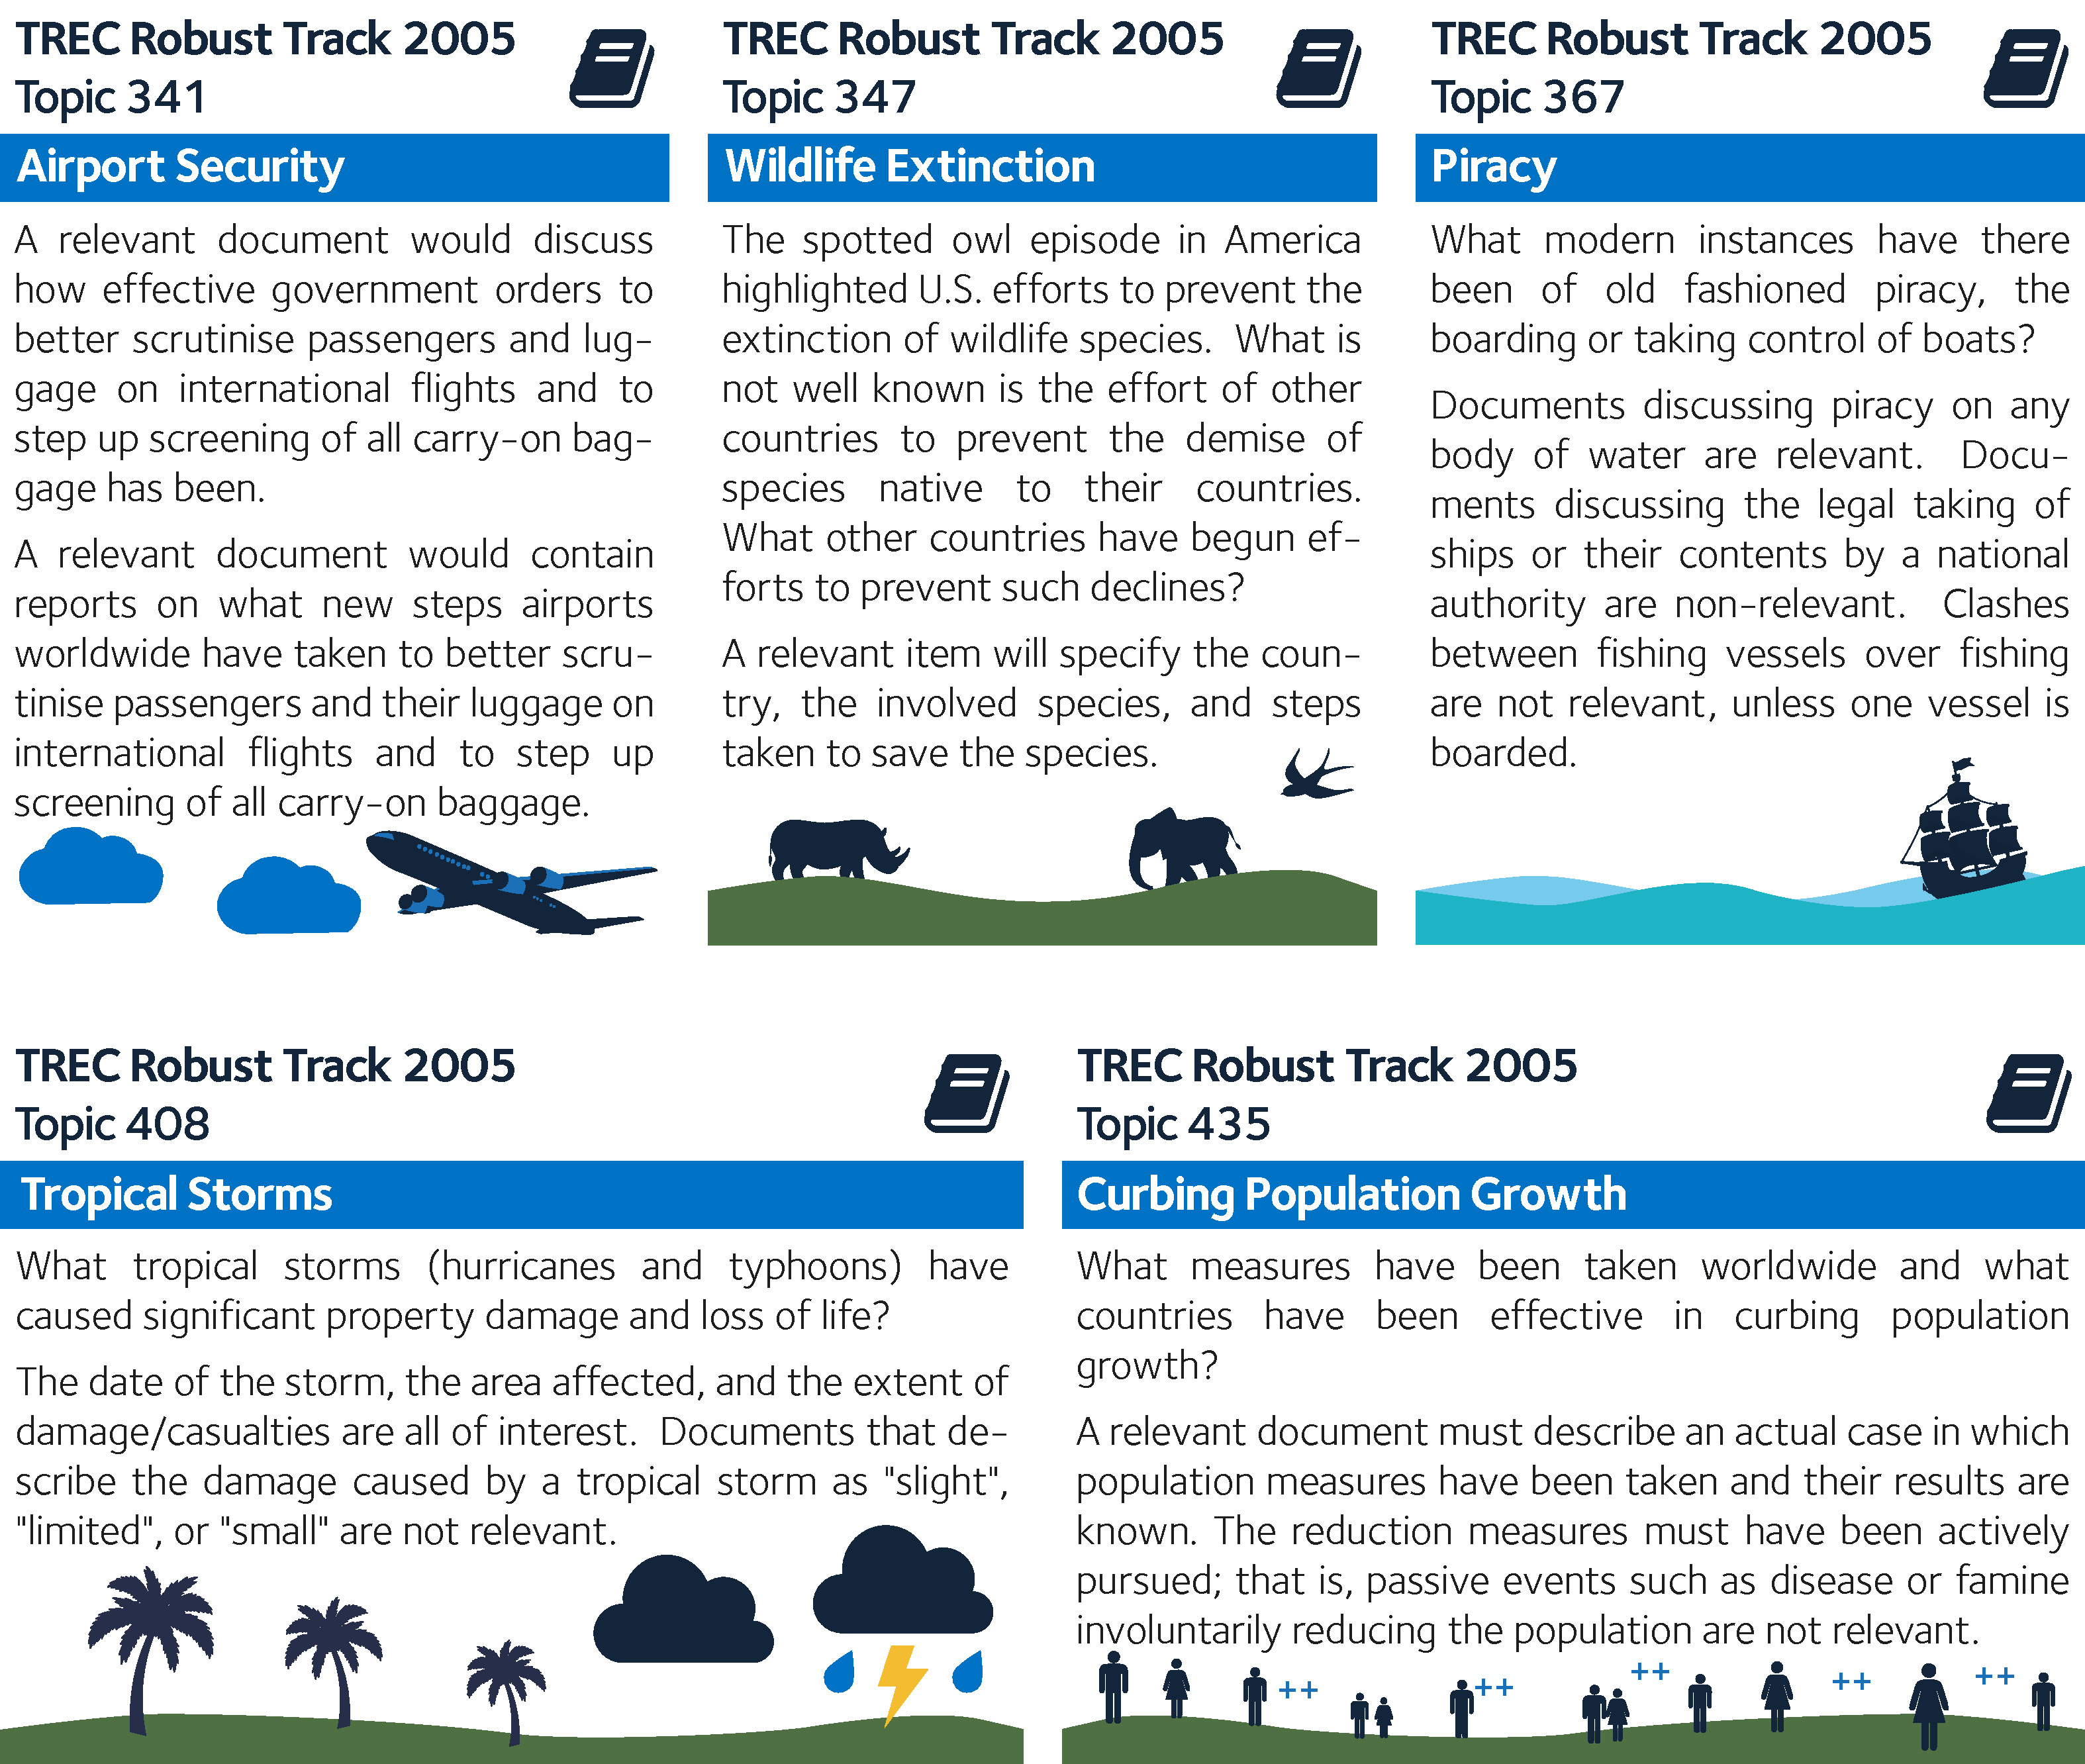
\includegraphics{figures/ch4-topics.pdf}}
    \caption[TREC topic titles and descriptions]{The titles and descriptions of the five~\gls{acr:trec} topics used in experimental work. Topics are extracted from the \emph{TREC 2005 Robust Track,} as outlined by~\cite{voorhees2006trec_robust}. Descriptions provide an explanation as to what constitutes a relevant (and often non-relevant) document.}
    \label{fig:topics}
\end{figure}

\subsection{Topics}\label{sec:methodology:collection:topics}
Five topics were also selected from the 50 provided in the \emph{TREC 2005 Robust Track,} as outlined by~\cite{voorhees2006trec_robust}. These topics are used throughout experimental work reported in this thesis, and were selected based upon evidence from a previous user study (of similar nature) conducted by~\cite{kelly2009user_study}. Evidence showed that the topics offered similar levels of difficulty. The five topics, along with a short description of what constitutes a relevant document, are listed below. These summaries are derived from the~\gls{acr:trec} topic descriptions that are provided as part of the~\gls{acr:trec} 2005 Robust Track. Figure~\ref{fig:topics} provides an illustration of the five topics, along with their descriptions. The remaining 45 topic descriptions are not used in this thesis.

\begin{itemize}
    
    \item{\blueboxbold{Topic 341 – Airport Security} This topic considers relevant documents as those that discuss additional security measures that were taken by international airports around the world. Relevance is only denoted when a document discusses measures that go beyond the basic passenger and carry-on luggage screening. For example, AQUAINT document \texttt{NYT19980616.0123} discusses \emph{San Francisco International Airport's} attempts at introducing a \emph{robot sniffer,} attempting to look for nitroglycerine in luggage.}
    
    \item{\blueboxbold{Topic 347 – Wildlife Extinction} As the title of the topic suggests, this topic concerns wildlife extinction, and what efforts have been taken by countries \emph{other than} the U.S. to counter the decline in endangered wildlife. Relevant documents explicitly mention the country, the species of animal, and the efforts the state or other governmental agency took to prevent decline in numbers. For example, document \texttt{XIE20000531.0205} discusses the breeding programme undertaken by China to bolster the number of Siberian Tigers in its jurisdiction.}
    
    \item{\blueboxbold{Topic 367 – Piracy} Instances of modern piracy are considered relevant to this topic -- not in the sense of software piracy, but the act of a water going vessel being boarded by individuals wishing to hijack it. Document \texttt{APW19980601.1065} provides an example of this -- the \emph{Petro Ranger}, a large fuel tanker, was boarded by pirates in 1998 in the South China Sea. To be relevant to the topic, the name of the vessel and the body of water it was hijacked on must be mentioned -- those discussing instances of when states intercepted vessels are not relevant.}
    
    \item{\blueboxbold{Topic 408 – Tropical Storms} Documents discussing major tropical storms are to be considered relevant, where the storm is reported to have caused significant damage and a large number of casualties. This is a particularly timely topic for the document corpus considered, as the 1998 hurricane season in the Caribbean has been reported to be one of the most costly -- both in terms of damage caused and lives lost -- in history.\footnote{This is reported by the US \emph{National Oceanic and Atmospheric Administration (NOAA),} as seen at \url{http://www.outlook.noaa.gov/98hurricanes/}. \urlaccessed{2018-05-18}} Document \texttt{APW19980921.1265} for example discusses the effects on Puerto Rico of Hurricane Georges in September 1998, leaving -- at the time of reporting -- three dead, many houses damaged, and thousands homeless.}
    
    \item{\blueboxbold{Topic 435 – Curbing Population Growth} The final topic considers efforts that have been made by countries around the world to control the ever increasing human population. Documents discussing this issue are only relevant to the topic if the results to a case have been made public, and a reduction in population has been actively pursued. The document must mention the country, the As such, events like famines are not relevant. A perhaps well known example of such a phenomenon is the one child policy that was pursued by China in the late 20\textsuperscript{th} century. Document \texttt{NYT19981031.0070} discusses the Chinese government's efforts to curb its expanding population at the time, with sexual education and heavy financial penalties for additional children. These efforts were shown to lead to a reduction in population, although whether this actually occurred is open to debate.}
    
\end{itemize}

For all user studies reported in this thesis, we selected topic \blueboxbold{367} as a \emph{practice topic,} permitting the participating subjects to familiarise themselves with the experimental system used. As such, we do not report any results from interactions that took place with this topic when reporting user studies. In the next section, we outline the different search tasks that were undertaken by user study subjects while using the aforementioned topics.

\section{User Study Methodology}\label{sec:methodology:user}
Using the aforementioned corpus, retrieval system and topics, we now move onto a discussion of the common methodology employed across two user studies. These are detailed in Chapters~\ref{chap:snippets} and~\ref{chap:diversity}. While intricate details of each study's methodology do indeed vary, these are nevertheless common components that we discuss in this section. As a reminder, the two studies examine:

\begin{itemize}
    \item{the length (and thus quality) of snippets presented in result summaries are varied (Chapter~\ref{chap:snippets}, conducted between July and August, 2016); and}

    \item{the overall search goal (time constraints vs. relevancy accruement) and task goal (ad-hoc vs. diversified results) are changed (Chapter~\ref{chap:diversity}, conducted in January, 2018).}
\end{itemize}
\vspace*{-4mm}

Specifically, the methodology used for these studies allowed us to determine how the stopping behaviour of a searcher varies when these conditions are varied. We discuss the specific interfaces and conditions that we trialled in subsequent chapters of this thesis.

Both user studies were undertaken using a custom built experimental framework called \blueboxbold{TREConomics}.\footnote{\treconomics~can be found online at \url{https://github.com/leifos/treconomics}. \urlaccessed{2018-05-15}} The pure-\emph{Python} framework has been developed over a number of years. It permits for straightforward deployment of~\gls{acr:iir}-based studies that have examined a variety of different aspects. It has been successfully deployed in a number of prior works, including those by:~\cite{azzopardi2013query_cost, maxwell2014temporal_delays, kelly2015serp_size, edwards2015query_interface}; and~\cite{crescenzi2016time_constraints}.

% Diversity study -- ethics number 622, Computer and Information Sciences Ethics Committee, University of Strathclyde.

\subsection{Experimental Details and Flow}\label{sec:methodology:user:flow}
Each user study was designed to last for approximately 45-50 minutes, including the completion of requested search tasks and surveys. Both experiments followed a similar structure, where subjects would complete a number of surveys before beginning a search task, and completing a further survey upon completion of the task. These surveys, as discussed in Section~\ref{sec:methodology:extracting:user}, permitted us to gather a series of usability measures (refer to Section~\ref{sec:ir_background:evaluation:user}) about the perceived experiences of subjects of the various interfaces and conditions.

The basic structure of both user studies was as follows.

\begin{itemize}
    \item[~\raisebox{-.2\height}{
\includegraphics[height=5mm]{figures/ch2-point1.pdf}}]{Subjects began by reading the experiment briefing sheet, before agreeing to continue.}
    \item[~\raisebox{-.2\height}{
\includegraphics[height=5mm]{figures/ch2-point2.pdf}}]{A demographics survey was then completed.}
    \item[~\raisebox{-.2\height}{
\includegraphics[height=5mm]{figures/ch2-point3.pdf}}]{Subjects then attempted the \emph{practice task,} using the practice topic. This allowed subjects to familiarise themselves with the system and its interface.}
    \item[~\raisebox{-.2\height}{
\includegraphics[height=5mm]{figures/ch2-point4.pdf}}]{Subjects would then complete the various search tasks set out for them. Each task consisted of three steps:}
    
    \begin{itemize}
        \item{a pre-task survey, capturing a subject's prior knowledge about the topic;}
        \item{the search task itself; and}
        \item{a post-task survey, capturing the subject's experiences regarding searching for information about the topic.}
    \end{itemize}
    
    \item[~\raisebox{-.2\height}{
\includegraphics[height=5mm]{figures/ch2-point5.pdf}}]{Upon completion of each search task, subjects would then complete a post-experiment survey, asking general questions about their experience across all the different tasks.}
    \item[~\raisebox{-.2\height}{
\includegraphics[height=5mm]{figures/ch2-point6.pdf}}]{Finally, upon completion, subjects would be presented with a results screen, providing a summary of their performance. Performance for each subject was presented on a per-task basis. After this information had been processed, the experiment concluded.}
\end{itemize}

Subjects undertook a total of four search tasks in which interactions and experiences were captured. Including the practice task at the beginning of each experiment, this took the total number of search tasks per subject up to five. Following a \blueboxbold{within-subjects study design}, the four search tasks -- each using a different topic as described in Section~\ref{sec:methodology:collection:topics} -- permitted us to trial each experimental condition/interface. The topics and tasks were assigned to subjects using a Latin-square rotation to minimise ordering effects. A within-subjects design increases the statistical power -- the number of `subjects' is higher than a between-subjects design. Limitations can consider issues such as fatigue. By being considerate of the time spent by subjects searching, fatigue for example could be limited.

\subsection{Experimental Search Interface}\label{sec:methodology:user:interface}
In this section, we discuss the experimental search interface that was used by subjects of the user studies.\footnote{Slight modifications to the search interface were made to the goal-based study, as we discuss in Section~\ref{sec:diversity:users:method}.} The interface would be familiar to anyone who had used a web-based retrieval system, and thus the learning curve for using the interface would most likely be low. Upon commencement of the experiment, the interface would launch in a fixed-size popup window (refer to Section~\ref{sec:methodology:user:crowdsourcing:technical}) of the web browser being used.

The interface consists of three main views, the two most important being shown in Figure~\ref{fig:interfaces}. The views were:

\begin{itemize}
    \item{the~\glsfirst{acr:serp}, presenting the query box and results for an issued query;}
    \item{the \emph{document view,} providing the source text of a documents; and}
    \item{the \emph{saved documents list,} providing a list of the documents that subjects had identified as relevant.}
\end{itemize}

In addition to the three views above, we also provided a \emph{topic view,} which, when requested, would open a further popup window that contained a description of the topic. This was purely to serve as a reminder, as subjects were provided the topic description in full before the search task began.

Common to all views was the inclusion of the blue navigation bar at the top of the popup window. As we discuss further in Section~\ref{sec:methodology:user:crowdsourcing:technical}, this bar was included to provide a series of different navigational links, such as, when on the document view page, a link to return to the originating~\gls{acr:serp}. Where applicable, we also provided a link for the subject to end the search task, if he or she felt that they had satisfied the criteria for the task.

\begin{figure}[t!]
    \centering
    \resizebox{1\hsize}{!}{
    
\includegraphics[width=1\textwidth]{figures/ch6-interfaces.png}}
    \caption[Example screenshots of the experimental interfaces]{Example screenshots of the basic search interface used as part of \treconomics. On the left is a screenshot of typical experimental~\gls{acr:serp} for the query \texttt{wildlife extinction}. The right shows the document view, showing the option for subjects to \texttt{Save} a document that they consider relevant to the given topic.}
    \label{fig:interfaces}
\end{figure}

\subsubsection{The SERP}\label{sec:methodology:user:interface:serp}
As can be observed from the left screenshot in Figure~\ref{fig:interfaces}, the~\gls{acr:serp} does not look all that different from a~\gls{acr:serp} on a contemporary web search engine -- sans right rail components, as we discussed previously in Section~\ref{sec:ir_background:user:iir:serp}. The experimental~\gls{acr:serp} provides at the top the \emph{query box,} allowing subjects to enter their query term(s), and a button to submit their query. The \texttt{ENTER} key could also be used to submit a query.

Once submitted, results are displayed underneath the query box. The issued query is provided, along with an approximation of how many pages of results are provided to the searcher for the given query. This hints that pagination is utilised -- with 10 results per page shown. At the bottom of each~\gls{acr:serp} are links that allow the searcher to move to the previous and next page of results.

\begin{figure}[h]
    \centering
    \vspace{4mm}
    \resizebox{1\hsize}{!}{
    
\includegraphics{figures/ch6-buttons.pdf}}
    \label{fig:serp_buttons}
    \vspace{-5mm}
\end{figure}

Result summaries were shown as discussed in Section~\ref{sec:ir_background:user:iir:serp}. The title, the source, and any snippet text were all provided. Given that the experiments were based upon news search, the source is the name of the newswire from which the document originates. The title was also hyperlinked.

\begin{figure}[h]
    \centering
    \vspace{0mm}
    \resizebox{1\hsize}{!}{
    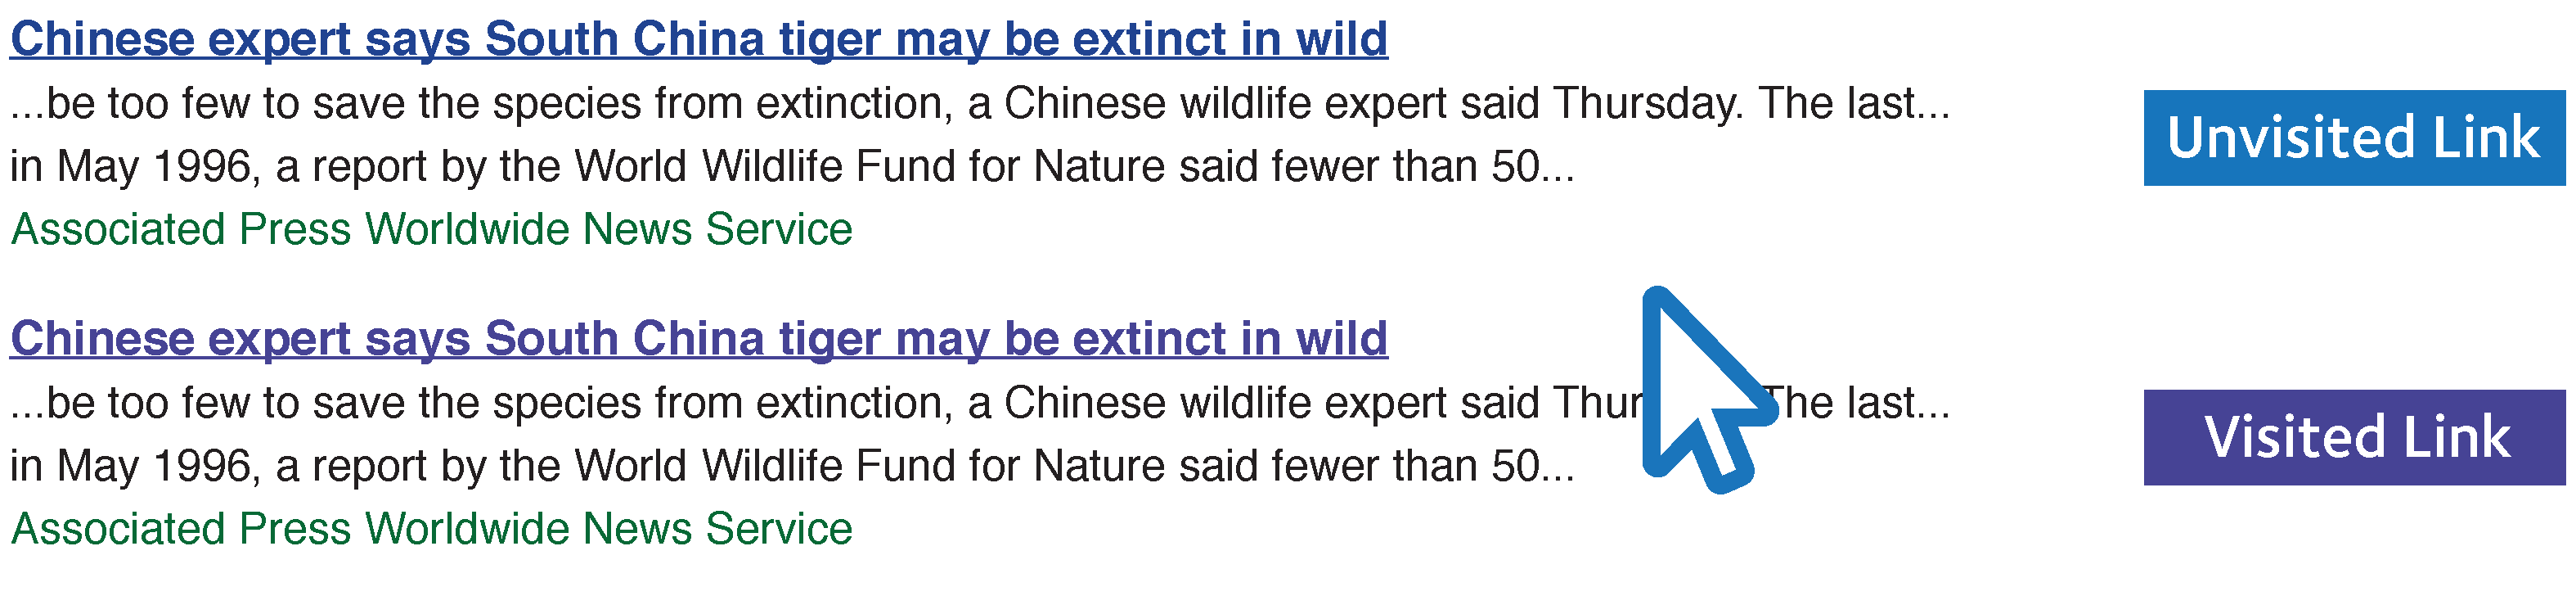
\includegraphics{figures/ch6-links.pdf}}
    \label{fig:serp_links}
    \vspace{-13mm}
\end{figure}

When a subject clicked on the link, he or she would then be taken to the document view (discussed below), displaying the associated document in its entirety. Standard hyperlink colours were employed -- blue for unvisited, and purple for visited. Examples of these link colours are shown above.

\subsubsection{The Document View}\label{sec:methodology:user:interface:document}
The right screenshot in Figure~\ref{fig:interfaces} illustrates the document view. The view provides the title, the document source (newswire), the date at which the document was created, and the full text of said document. On the right rail of the page, subjects were provided with two buttons -- one to return them to the originating~\gls{acr:serp}, or another to \emph{save} the document. The act of saving a document is a crucial component to both studies we discuss in this thesis. It provided us with a mechanism to determine what documents subjects thought were relevant to the given topics. This mechanism for instance also provided us with a means to calculate a subject's performance.

\subsubsection{The Saved Documents View}\label{sec:methodology:user:interface:saved}
The third key view, as mentioned above, allowed subjects to view a list of documents that they had previously saved as relevant to the given topic. This list of documents also provided buttons, allowing subjects to change their decisions as to what constituted as a relevant document. We provided this functionality as~\gls{acr:iir} is inherently an interactive process -- a searcher \emph{learns} and develops their mental model of the given information need as more information is presented to them~\citep{ingwersen2005theturn}.

\subsection{Capturing Interactions and Survey Responses}\label{sec:methodology:user:capturing}
In addition to the interface, the \treconomics~framework provided extensive logging capabilities to capture a variety of different events triggered by subjects as they performed search tasks. This resulted in the generation of an experiment \emph{log file,} capturing the date, time, searcher and topic for each event that was logged. Figure~\ref{fig:log} provides an anonymised excerpt from the interaction log of the user study presented in Chapter~\ref{chap:snippets}.

The figure illustrates the different actions that were logged from when a searcher begins interactions with the query box (\texttt{QUERY\_FOCUS}), to issuing a query (\texttt{QUERY\_ISSUED}, complete with the terms of the query), to clicking a document (\texttt{DOC\_CLICKED}), and, finally, to saving the document (or considering it relevant to the given topic, \texttt{DOC\_MARKED\_RELEVANT}). A detailed discussion of the different behavioural measures that we examined from the interaction log are detailed in Section~\ref{sec:methodology:extracting}.

\begin{figure}[t!]
    \centering
    \resizebox{1\hsize}{!}{
    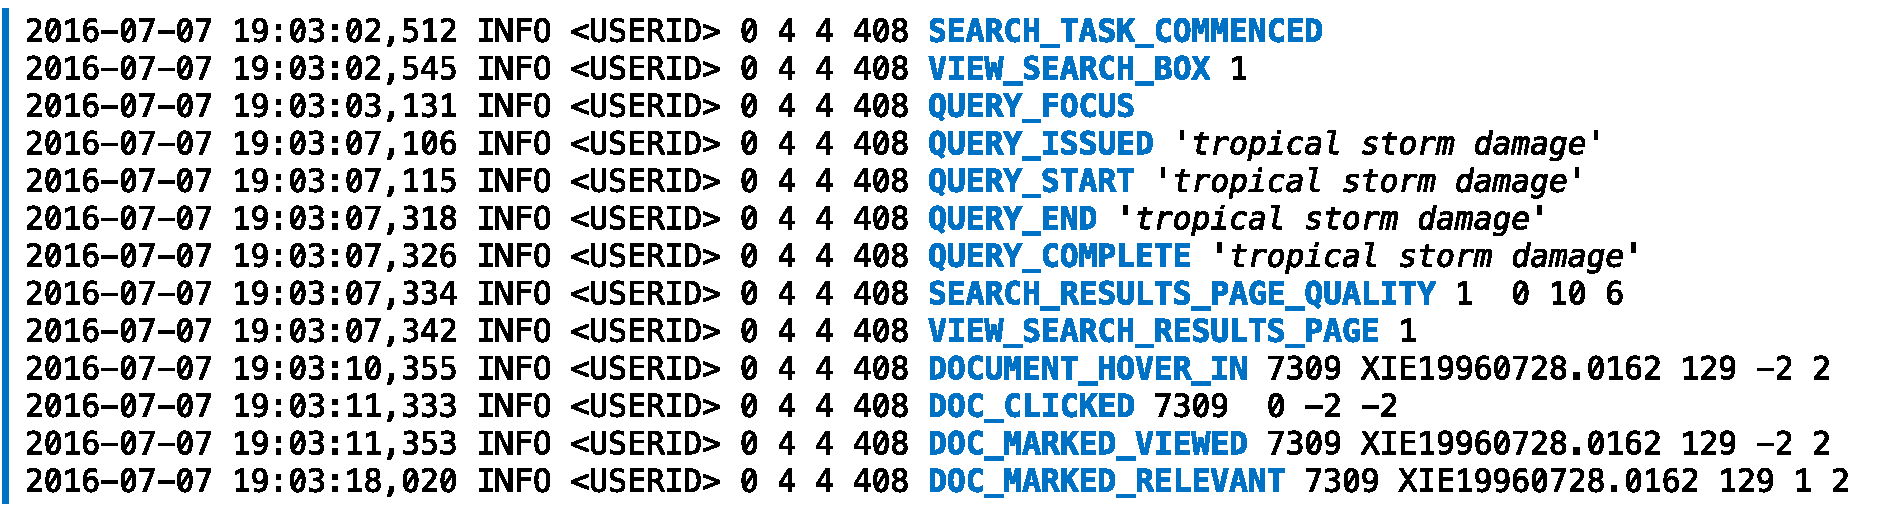
\includegraphics{figures/ch6-log.pdf}}
    \caption[Experiment log file excerpt]{An excerpt from the interaction log of the user study detailed in Chapter~\ref{chap:snippets}. A sequence of interactions are shown that were logged by the \treconomics~framework.}
    \label{fig:log}
\end{figure}

The \treconomics~framework also saved the responses from surveys as completed by the subjects of each study. These were saved to a separate~\gls{acr:rdbms}, with a number of scripts subsequently created to extract and analyse the saved responses.

\subsection{Crowdsourcing Considerations}\label{sec:methodology:user:crowdsourcing}
An important factor in planning any user study is the economics of collecting input from subjects. \emph{Where do the subjects come from? How do we recruit them?} A traditional, lab-based study as discussed in Section~\ref{sec:ir_background:user} typically involves a significant investment in time and monetary cost from the researchers conducting the experiment~\citep{spool2001testing}. For both user studies previously detailed, we employed a \emph{crowdsourced} approach to our experimentation. Crowdsourcing is the practice of obtaining input into a task by enlisting the services of a number of people, recruited over the Internet.

As highlighted by~\cite{zuccon2013crowdsourcing_comparisons}, crowdsourcing provides an alternative means for capturing user interactions and search behaviours. Greater volumes of data can be obtained from more heterogeneous workers at a lower cost -- all within a shorter timeframe. Of course, pitfalls of a crowdsourced approach include the possibility of workers completing tasks as efficiently -- but not effectively -- as possible, or submitting their tasks without performing the requested operations~\citep{feild2010turkers}.

Despite these issues, it has been shown that there is little difference in the quality between crowdsourced and lab-based studies~\citep{kely2011user_study, zuccon2013crowdsourcing_comparisons}. Nevertheless, quality control is a major component of a well-executed crowdsourced experiment, with examples in a similar research area including work by~\cite{kazai2011crowdsourced} and ~\cite{crescenzi2013crowdsourced}.

Using crowdsourcing for the two user studies, we detail in the remainder of this section the precautions that were taken during, discussing both the requirements for the subjects and their technical setup -- as well as a discussion of the crowdsourcing platform used.

\subsubsection{Platform Details}\label{sec:methodology:user:crowdsourcing:platform}
Both studies were run over the~\glsfirst{acr:mturk} platform. Workers\footnote{In this section, a \emph{worker} refers to an individual undertaking the experiment on the MTurk platform. This term is considered interchangeable with a \emph{subject.}} from the platform each performed a single task (or, to use MTurk language, a \emph{Human Intelligence Task (HIT)}), with a single HIT corresponding to the entire experiment. This is in contrast to many other crowdsourced studies, where workers would typically undertake small -- typically decision-based -- HIT transactions.

\subsubsection{Subject Requirements}\label{sec:methodology:user:crowdsourcing:subjects}
Due to the expected length that workers would take to complete the two studies\footnote{Note that two different sets of workers were used -- the studies were run at different times.}, workers who completed the study in full were reimbursed for their time with US\$9 -- greater than the hourly minimum wage set by the US federal government. Workers interested in undertaking each of the two studies were required to meet a certain minimum set of criteria to be eligible to participate. We required that workers were:

\begin{itemize}
    \item{from the U.S.;}
    \item{native English speakers;}
    \item{possessed a HIT acceptance rate of at least 95\%; and}
    \item{had at least had 1000 prior HITs approved.}
\end{itemize}

Requiring a high HIT acceptance rate reduced the likelihood of recruiting workers who would not complete the study in a satisfactory manner. Recruits were forewarned about the length of the HIT, providing them with a chance to abandon the experiment if they felt the expected time was too long.

\subsubsection{Technical Requirements}\label{sec:methodology:user:crowdsourcing:technical}
Given worker limitations, we also enforced a number of technical constraints. Workers attempting each experiment were required to have a sufficiently large computer screen to display the experimental interface without having to resort to excessive scrolling, and ensured a consistent number of result summaries would be present on different worker's screens. As such, we imposed a minimum display resolution of $1024x768$ for both studies. 

Conducted through a web browser, we wanted to ensure that only the controls provided by the experimental apparatus were used, meaning that the popup window that we highlighted in Section~\ref{sec:methodology:user:interface} had all other browser controls disabled to the best of our ability (i.e. browser history navigation, etc.). The experimental system was tested on several major web browsers (including \emph{Google Chrome, Mozilla Firefox,} \emph{Apple Safari} and \emph{Microsoft Edge)}, across different operating systems (including \emph{Microsoft Windows,} \emph{Apple macOS} and several \emph{Linux} distributions, focusing on \emph{Ubuntu)}. This gave us confidence that a similar experience would be had across different system configurations.

\section{Extracting User Study Data}\label{sec:methodology:extracting}
As discussed in Section~\ref{sec:methodology:user:capturing}, the \treconomics~framework provided the necessary infrastructure for us to log the various interactions and capture survey responses from each individual subject across the two user studies trialled. In this section, we provide details on the different aspects that we subsequently used to evaluate searcher behaviours, performance and user experience. Figure~\ref{fig:evaluation_methodology} provides a graphical illustration of how we split the various aspects we consider into four distinct categories.

The first three categories can be extracted directly from the interaction log that recorded different interactions by each subject as they progressed through the experiment. The categories we considered are listed below.

\begin{itemize}
    
    \item{\blueboxbold{Behavioural Measures} capture the broad interactions that take place, such as the number of documents that a searcher examined in detail.}
    \item{\blueboxbold{Performance} measures could then be extrapolated, with aid of~\gls{acr:trec} QREL relevance judgements, to ascertain the performance of subjects.}
    \item{\blueboxbold{Time-Based} measures can also be derived from directly examining the interaction log, measuring the time spent between different logged interactions.}
    
\end{itemize}

In addition to these categories, we also considered a number of \blueboxbold{user experience} measures that were derived from a series of surveys. As highlighted in Section~\ref{sec:methodology:user:flow}, surveys were presented to subjects at a number of different stages throughout the experiment. In conjunction with the three log-based categories defined above, the user experience measures could be used to complement the empirical evidence to see whether the interactions of subjects actually correlated with their perceived experiences.

In all, the interactions -- including aspects such as clicks, and time-based measures, were used as a \emph{grounding} for our subsequent user simulations of interaction. How we grounded these simulations is discussed in Section~\ref{sec:method:simulation:grounding}.

\begin{figure}[t!]
    \centering
    \resizebox{1\hsize}{!}{
    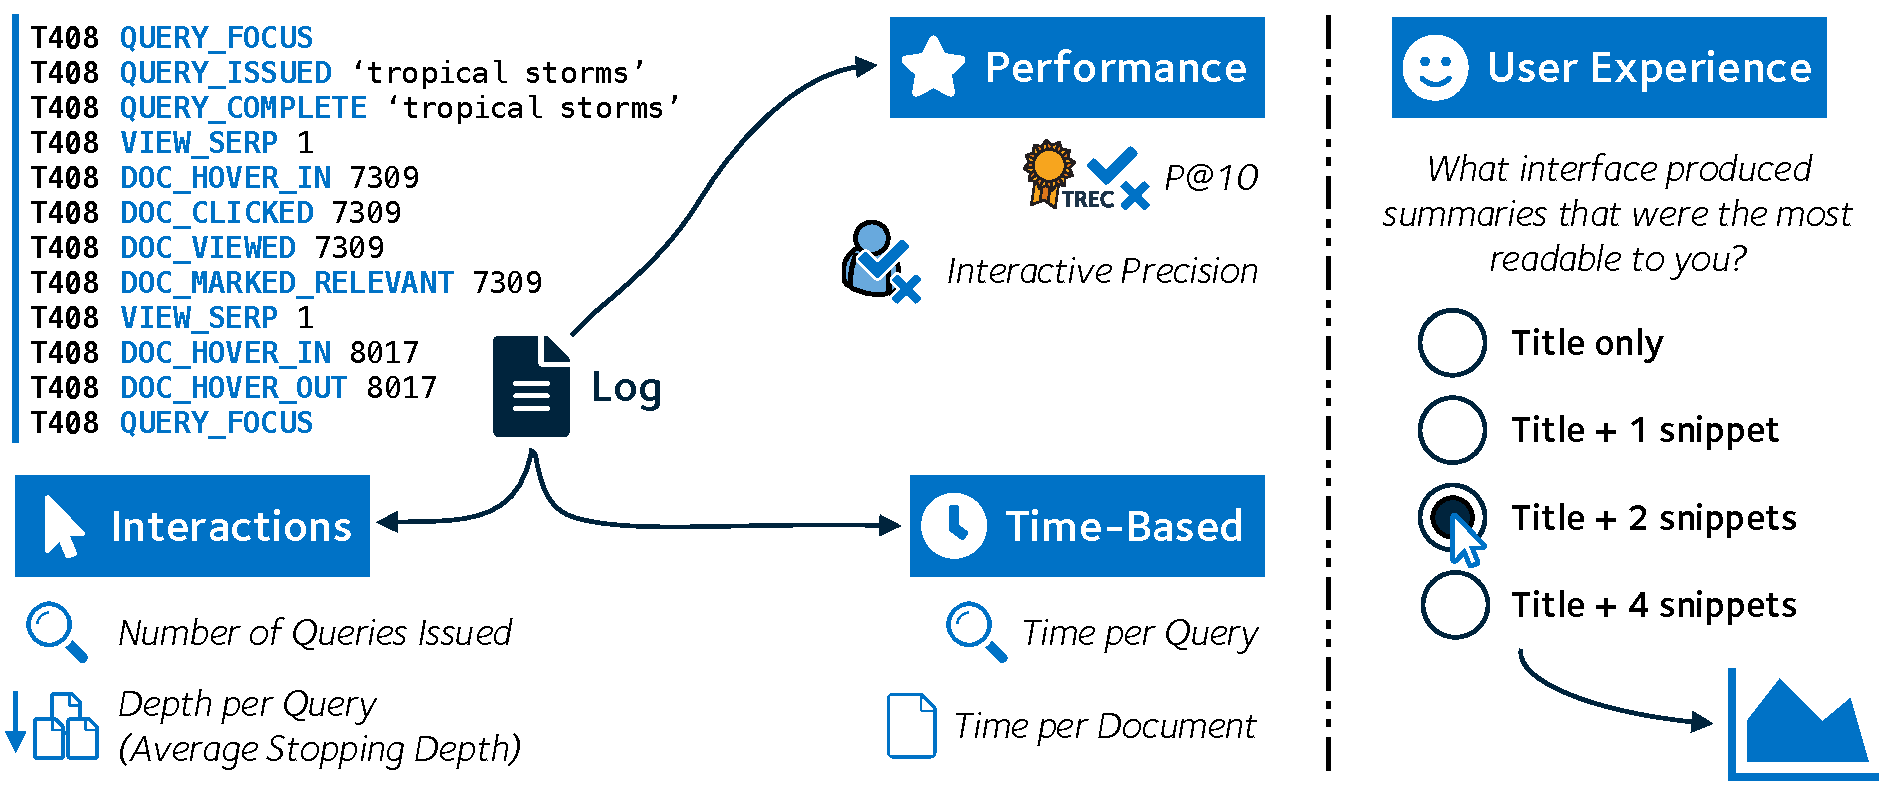
\includegraphics{figures/ch4-evaluation.pdf}}
    \caption[Examples of evaluation measures]{An illustration of the different types of measures that are captured, and from what sources. Interaction, time-based and performance measures are derived from the user study experiment log (with~\gls{acr:trec} QRELs used in conjunction with the interaction log to compute a subject's performance). User experience metrics are collated from a number of different surveys. Refer to Section~\ref{sec:methodology:extracting} for more information.}
    \label{fig:evaluation_methodology}
\end{figure}

\subsection{Behavioural Measures}
Recorded solely from interaction log data, the basic interactions covered a large proportion of the aspects we considered in our analyses. They key behavioural measures we examined are listed below.

\begin{itemize}
    \item{\blueboxbold{Queries} We considered the number of queries that had been issued.}
    \item{\blueboxbold{Documents} The number of documents that were examined (viewed).}
    \item{\blueboxbold{\glsplural{acr:serp}} The number of~\glsplural{acr:serp} that were examined.}
    \item{\blueboxbold{Examination Depth} The depth to which subjects clicked on (and hovered over) result summaries on the associated~\glsplural{acr:serp}.}
\end{itemize}

From these measures, we could then ascertain whether searcher behaviour varied when a certain condition or interface was changed -- allowing us to address questions such as \emph{whether snippet length affects the depth to which searchers examine content?} To compute depths, click and hover depths were used -- we however only report click depths in subsequent contributory chapters. The reasoning for this is discussed in Section~\ref{sec:methodology:extracting:time} below. These measures were computed over each query issued by the different subjects.

% -- we could then take an average for each subject. We could go even further, too -- averaging over each topic, interface or condition as required to observe any notable trends in behavioural changes.

\subsection{Time-Based Measures}\label{sec:methodology:extracting:time}
As discussed in Section~\ref{sec:methodology:user:capturing} -- and also illustrated in Figure~\ref{fig:log} on page~\pageref{fig:log}, each logged interaction was saved with a timestamp which allowed us to determine when each event occurred.\footnote{Timestamps were saved to the nearest thousandth of a second, as per the specification of the standard Python logging framework -- refer to \url{https://docs.python.org/2/howto/logging-cookbook.html} \urlaccessed{2018-05-29} for an example of the framework in action.} With these timestamps, we could then measure the time between two associated events, thus yielding the time taken to perform a given activity. We considered five key time-based measures across both user studies that we enumerate below, along with a description of the log events that we measure each time from.

\begin{itemize}
    \item{\blueboxbold{Queries} This measure considered the time spent by a searcher issuing queries to the retrieval system. This is captured from the point at which the searcher focuses upon the query box (\texttt{QUERY\_FOCUS}) to the point at which the query is submitted (via the \texttt{QUERY\_ISSUED} event, either by pushing the \emph{Search} button or the subject pushing \Return on their keyboard).}
    \item{\blueboxbold{\gls{acr:serp} Content} This measure considers the total amount of time that a searcher spends on a given~\gls{acr:serp}. This is captured as the point at which the subject is presented with the~\gls{acr:serp} itself (\texttt{VIEW\_SEARCH\_RESULTS\_PAGE}) to the point at which they leave -- either through the issuance of a further query, clicking on a document hyperlink, or navigating to one of the other views of the experimental interface.}
    \item{\blueboxbold{Result Summaries} As discussed below, this is the mean time spent by a subject examining individual result summaries on a given~\gls{acr:serp}. As such, this is included within the~\gls{acr:serp} content time.}
    \item{\blueboxbold{Documents} This measure considers the time a subject spends on the document view. This is captured as the point at which the document is presented on the subject's screen (\texttt{DOC\_MARKED\_VIEWED}) to the point at which they leave, which, like the~\gls{acr:serp} content time, could be determined from a number of different events.}
\end{itemize}

The fifth time-based measure that we considered in our reporting of results was an amalgamation of the four listed above.

\begin{itemize}
    \item{\blueboxbold{Total Session Time} The total session time is the addition of each of the time times measured above. This is essentially the same as the time from the very first \texttt{QUERY\_FOCUS} event to the \texttt{TASK\_COMPLETED} event, which is either triggered by an interface timeout (Chapter~\ref{chap:snippets}) or the subject ending the task herself or himself (Chapter~\ref{chap:diversity}).}
    
\end{itemize}

It should be noted that in this thesis \blueboxbold{we report all durations in seconds}. We considered a number of different approximations when measuring each of the above. For example, the querying time is measured only as the time the searcher spends interacting with the query box. Subjects may well have spent longer considering what terms to enter, perhaps as they were browsing existing content. However, this could be not captured; out logging tools were not capable of capturing this additional time.

A further approximation used was the time per result summary. This was computed by dividing by the click depth reached on a given~\gls{acr:serp} by the duration between the first \emph{hover} event, where the subject hovered his or her cursor over a result summary, and the time at which they left the~\gls{acr:serp}. The first hover event was chosen as it was deemed to be a good indicator of the beginning of interaction with result summaries. The mouse cursor has been shown in prior studies to correlate strongly with the subject's gaze on the screen~\citep{chen2001mouse_cursor, smucker2014judging_relevance_movements}. However, issues with network latency meant that several of the hover events were logged in the incorrect order, making the approach of measuring each individual \texttt{HOVER\_IN} and \texttt{HOVER\_OUT} event unreliable. Using the click depth and total~\gls{acr:serp} time provided us with an approximation with which to work with. The approximation also makes an assumption that subjects examined each result summary on a~\gls{acr:serp} up to a particular depth, for an equal period of time. This was sufficient for the work in our study to ascertain whether or not a variation in the task goal or presentation of results affected the depths to which subjects examined results.

These time calculations and approximations were also used as a means for providing \emph{grounding} to the simulations of interaction, as we discuss later in Section~\ref{sec:method:simulation:grounding:costs}. It should also be noted that the time per interaction could also be computed, such as the \emph{time per query.} This was simply considered as the summation of the querying time across the entire session, for example, divided by the total number of queries issued. The same principle could be applied for the \emph{per~\gls{acr:serp} time} and the \emph{per document time.}

\subsection{Performance Measures}\label{sec:methodology:extracting:performance}
In conjunction with behavioural and time-based measures, we were also able to extract a number of different performance measures from the interaction logs.\footnote{Some measures were computed with the \texttt{trec\_eval} evaluation tool, discussed in Section~\ref{sec:ir_background:paradigms:trec}.} Key performance measures that we captured included:

\begin{itemize}
    \item{\blueboxbold{query performance}, primarily measured with $P@10$ (although additional $P@k$ values are reported); and}
    \item{\blueboxbold{interactive precision and recall} (as discussed in Section~\ref{sec:ir_background:evaluation:user:ipr}), including:}
    
    \begin{itemize}
        \item{the number of documents saved (identified as relevant); and}
        \item{the number of those documents that were~\gls{acr:trec} relevant (and vice-versa).}
    \end{itemize}
\end{itemize}

\blueboxheader{Grounding Subsequent Experiments} With behavioural measures and time-based measures in particular, these could be then used to \emph{ground} subsequent simulations of interaction. Refer to Section~\ref{sec:method:simulation:grounding} for further information on how this was achieved. The above measures were however sufficient for analysing how searcher behaviour changed.

\subsection{Demographics and User Experience Surveys}\label{sec:methodology:extracting:user}
A number of surveys were also filled out by subjects. These captured different information about each searcher's individual search experiences. While there are similarities between what is asked (refer to Sections~\ref{sec:snippets:method} and~\ref{sec:diversity:users:diversifying} for further details), we in this section provide a high-level overview of the different surveys, before examining questions that were common between the two. We break these overviews into three sections, in the order of the experimental flow detailed in Section~\ref{sec:methodology:user:flow} -- demographics, pre- and post-task surveys, and post-experiment surveys.

\subsubsection{Demographics}
Details in keeping with general demographics were attained about the different subjects from this survey. These included the following basic demographic questions:

\begin{itemize}
    \item{the subject's age and gender;}
    \item{their present occupation; and}
    \item{their highest level of professional qualification (e.g. high school, Honours, MSc or PhD).}
\end{itemize}

In addition to these basic questions, we also asked several questions pertaining to their perceived search proficiency. Questions included:

\begin{itemize}
    \item{how often they searched for information;}
    \item{how often they search for news articles (being a news-based experiment);}
    \item{what pointing device they were using (i.e. mouse, trackpad); and}
    \item{their preferred general purpose web search engine.}
\end{itemize}

Considering that both experiments considered the news searching domain, we asked each subject how often they searched for news articles online.

\subsubsection{Pre-Task}
Between both user studies, we asked the same questions within the pre-task survey. Subjects were provided with a short description of their search task and a topic description, providing their information need for said task. After examining the topic description, subjects were then queried on the following:

\begin{itemize}
    \item{how well they knew about the topic prior to this study;}
    \item{how relevant the topic was to their life;}
    \item{how interested they were to learn more about the topic;}
    \item{whether they had searched for information related to the topic before; and}
    \item{how difficult they felt it would be to search for information on the topic before commencing.}
\end{itemize}

Responses were provided on a seven-point scale, providing the option for neutrality between the two extremes -- extremes being \emph{nothing/not at all/very difficult} to \emph{lots/very much/very easy.} Responses to these questions helped us gauge the perceived difficulty of the task, and ascertain how much background knowledge could potentially affect results.

\subsubsection{Post-Task and Post-Experiment}
Post-task and post-experiment surveys were unique to each of the two user studies. Sections~\ref{sec:snippets:method} and~\ref{sec:diversity:users:diversifying} provide further information on what questions were asked. However, the post-task surveys focused on how well the subjects thought they (and the retrieval system, under the given condition and/or interface) performed during the search task. Post-task surveys considered the experiment as a whole, asking questions about what condition and/or interface the subjects preferred, or performed more to their liking, for example.

\section{Simulating Searcher Behaviours}\label{sec:method:simulation}
With the general layout and components of the two user studies explained, we now consider how we \emph{simulated searcher behaviours.} The simulation of interaction provides a low-cost means for exploring a variety of different searcher strategies and configurations~\citep{azzopardi2010workshop}. In this section, we provide an overview of the general aspects of the \blueboxbold{stochastically-based} searcher simulations that we discuss the results of in subsequent chapters of this thesis. Specifically, we discuss in this section:

\begin{itemize}
    \item{how our simulations were \emph{grounded;} and}
    \item{how we instantiated the different components of the~\gls{acr:csm} defined in Chapter~\ref{chap:csm} for our simulation experiments.}
\end{itemize}

We conclude the chapter with a discussion as to how we evaluate the results from our simulations, allowing us to determine what stopping strategies offer the best overall performance and approximations of real-world searcher behaviours. This is done in consideration of the two user studies discussed in Chapters~\ref{chap:snippets} and~\ref{chap:diversity}. By grounding our simulations with data derived from the two aforementioned user studies, we can then obtain an insight into how searcher stopping behaviours vary under different contexts.

\blueboxheader{The Mean Searcher} Comparisons between simulations and real-world searcher approximations are made between the \emph{average} behaviours observed. This average behaviour is considered across each of the different experimental interfaces and conditions that we trial across the two user studies, discussed in Chapters~\ref{chap:snippets} and~\ref{chap:diversity}. This consideration:

\begin{itemize}
    \item{simplifies and reduces the number of simulations that are required to be run; and}
    \item{provides a simple overview of how stopping behaviour varies across each interface and condition, rather than across each individual searcher.}
\end{itemize}

\blueboxheader{Considering Stochastic Simulations} We consider a series of different \emph{stochastically-based} simulations that attempt to mimic searcher behaviours. Currently, a majority of research that considers the simulation of interaction are also stochastic in nature, utilising probabilistic models. For example,~\cite{carterette2011effectiveness_evaluation} simulated the interaction of users for the purposes of evaluation through a dynamic test collection. While not explicitly stated, the underlying model of their simulations followed a similar process to the~\gls{acr:csm} as described in Chapter~\ref{chap:csm}, and were instantiated with probabilistic components.~\cite{baskaya2013behavioural_factors}, as discussed in Section~\ref{sec:ir_background:user:models}, developed a Markov-based model of the search process, with changes in state determined by a series of different probabilities. A similar, probabilistic browsing model was also proposed by~\cite{yilmaz2010browsing_utility}. These models considered probabilistically determining, for instance, the attractiveness of a result summary to the given information need -- something that we also utilise. We discuss this further in Section~\ref{sec:method:simulation:grounding:judgements}.

\subsection{The SimIIR Framework}\label{sec:method:simulation:simiir}
All simulations that were run as part of this thesis were performed using the \simiir~framework, a custom built framework for the simulation of interaction within the wider~\gls{acr:iir} process~\citep{maxwell2016simiir}.\footnote{\simiir~can be accessed at \url{https://github.com/leifos/simiir}. \urlaccessed{2018-05-29}} The framework consists of a number of individual \emph{components,} each which must be instantiated to yield a \emph{simulation.} Figure~\ref{fig:simiir} provides an illustration of the framework's basic architecture, highlighting each of the individual simulator components and the framework's key outputs.

In this section, we briefly outline each of these components, discussing the need for each. Each of these components can be mapped to one of the individual decision points and/or activities of the \gls{acr:csm}, as outlined in Section~\ref{sec:csm:flow} on page~\pageref{sec:csm:flow}.

A \emph{simulation} within the \simiir~framework consists of the following main components.

\begin{itemize}
    \item{\blueboxbold{Topics} One or more topic(s) can be supplied, each consisting of a title and topic description (i.e. the~\gls{acr:trec} topic descriptions).}
    \item{\blueboxbold{Retrieval System} An interface is provided to retrieval system that is to be used with the experiment. In the case of this thesis, this links back to the setup described in Section~\ref{sec:methodology:collection:system}.}
    \item{\blueboxbold{Output Controller} This component is responsible for generating the output files that can be fed into evaluation programs such as \texttt{trec\_eval}, as outlined in Section~\ref{sec:ir_background:paradigms:trec}.}
\end{itemize}

\begin{figure}[t!]
    \centering
    \resizebox{1\hsize}{!}{
    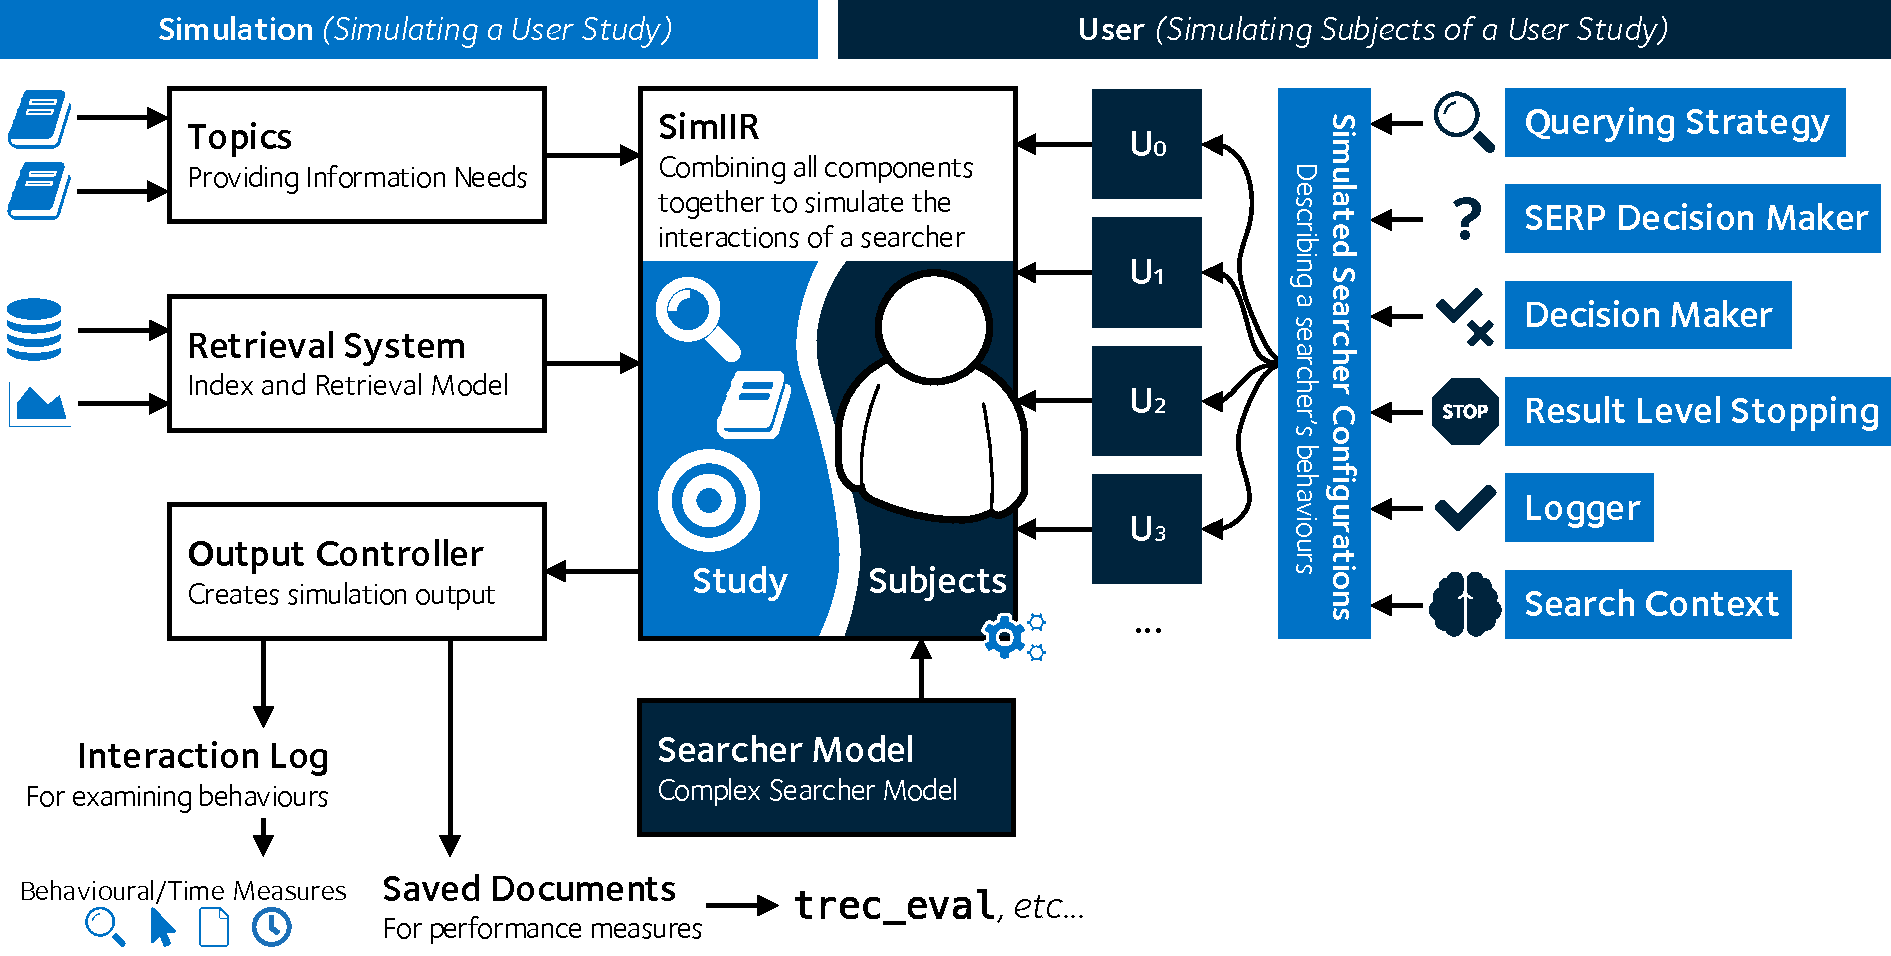
\includegraphics[width=1\textwidth]{figures/ch6-simiir.pdf}}
    \caption[SimIIR architecture]{The architecture of the \simiir~framework, with the components split across both \emph{simulation} and \emph{user} categories. Simulation components define the simulation – a representation of some real-world user study, with user components defining the behaviours of simulated searchers.}
    \label{fig:simiir}
\end{figure}

Simulations also consist of one or more \blueboxbold{simulated searchers}, which attempt to complete a given search task, having been instantiated with differing constraints. A simulation is therefore in essence loosely associated with the concept of a real-world \emph{user study.} Each individual searcher -- that can be likened to an individual subject of a user study -- consists of additional components that \emph{describe their behaviours.}

\begin{itemize}
    \item{\blueboxbold{Querying Strategy} The querying strategy determines how queries are generated from topic descriptions, and subsequently selected.}
    \item{\blueboxbold{\gls{acr:serp} Decision Maker} This decision maker determines where a searcher should \emph{enter} a~\gls{acr:serp} and begin to examine individual result summaries, or abandon the~\gls{acr:serp} and issue a subsequent query.}
    \item{\blueboxbold{Classifier/Decision Maker} These components are responsible for judging the attractiveness and relevancy of result summaries and documents respectively.}
    \item{\blueboxbold{Result Summary Level Stopping Strategy} This component, instantiated using one of the stopping strategies outlined in Chapter~\ref{chap:strategies}, determines the point at which a simulated searcher will stop interacting with a ranked list of results.}
    \item{\blueboxbold{Logger} The logger component is responsible for providing \emph{interaction costs} for particular interactions (e.g. issuing a query), keeping track of the combined session time, and determining whether the overall search session goal, time limit -- or other session level stopping constraint -- has been met.}
    \item{\blueboxbold{Search Context} This component can be considered as a basic representation of a searcher's brain, keeping track of the different result summaries and documents that have been examined, prior queries that have been issued, and what documents have been identified as relevant.}
\end{itemize}

All the above components are underpinned by a \blueboxbold{searcher model} component, providing a flow of interactions to the search process undertaken by simulated searchers. In all simulations reported in this thesis, this consists of the~\gls{acr:csm}. We do not discuss further details about how the \simiir~framework can be instantiated and used here; a high-level demonstration paper by~\cite{maxwell2016simiir} provides such a discussion.

\subsection{Grounding and Instantiating Simulations}\label{sec:method:simulation:grounding}
To ensure that the simulations of interaction are as realistic as possible, we \emph{grounded} said simulations using real-world observations extracted from interaction log data. Doing so ensures that the results of the simulations are credible~\citep{azzopardi2010workshop}. Given the~\gls{acr:csm}, we grounded the simulations of interaction from three main angles.

\begin{itemize}
    \item{\blueboxbold{Query Generation} We consider the generation of \emph{psuedo-realistic} queries to issue to the underlying retrieval system. As discussed in Section~\ref{sec:method:simulation:grounding:querying}, these queries are generated using \emph{querying strategies} that are created from observing real-world searcher querying behaviours.}
    \item{\blueboxbold{Interaction Costs} We extract a series of different interaction costs from log data to ensure that the time `spent' by simulated searchers is an average representation of the time spent by real-world searchers under a particular search context.}
    \item{\blueboxbold{Interaction Probabilities} As with interaction costs above, we also considered a series of grounded interaction probabilities that determine the likelihood of a simulated searcher determining whether to \emph{enter} a given~\gls{acr:serp}, the attractiveness of a result summary, or the relevance of a document.}
\end{itemize}

These are considered in conjunction with the twelve stopping strategies (as discussed in Chapter~\ref{chap:strategies}), and the various constraints that we imposed upon each searcher. The remainder of this section is left to detailed discussion of the key components of our simulations of interaction. In particular, this section focuses upon how we instantiated each of the individual components to yield realistic, credible results.

\subsubsection{Interaction Costs}\label{sec:method:simulation:grounding:costs}
Upon the examination of the~\gls{acr:csm}, illustrated in Figure~\ref{fig:csm} on page~\pageref{fig:csm}, a number of different \emph{interaction costs} can be derived. These are costs that must be expended by searchers subscribing to the model, in order for them to successfully complete the search process. In conjunction with the time-based measures discussed in Section~\ref{sec:methodology:extracting:time}, we identified five different interaction costs that searchers are faced with. These are listed below, with an illustration of the costs provided in Figure~\ref{fig:costs}.

\begin{itemize}
    \item{\blueboxbold{Querying} This considers the \emph{Issue Query} activity of the~\gls{acr:csm}, and considers the time required by a simulated searcher to enter a query into the retrieval system's interface. Again, this is considered as from when the subject focused on the query box, to the point where they submitted the query.}
    \item{\blueboxbold{\gls{acr:serp} Examination} This cost considers the \emph{View~\gls{acr:serp}} activity, and denotes the time spent by a searcher considering whether the presented~\gls{acr:serp} is attractive enough to \emph{enter} and examine in more detail. This is considered as the point at which the~\gls{acr:serp} is rendered on their screen, to the point where they begin interacting with it in any way.}
    \item{\blueboxbold{Result Summary Examination} The \emph{Examine Snippet} activity is considered here, this being the time required to examine an individual result summary for attractiveness. Estimations for this interaction cost are described in Section~\ref{sec:methodology:extracting:time}.}
    \item{\blueboxbold{Document Examination} This costs denotes the amount of time required to assess a document for relevance to the given information need. This is the \emph{Assess Document} activity.}
    \item{\blueboxbold{Saving} The \emph{Save Document} activity is considered for this final cost, where a searcher will actively save and identify the document as relevant. This is considered as the time from the point at which a searcher clicked the \emph{Save} button to when they left the document and returned to the~\gls{acr:serp}.}
\end{itemize}

\begin{figure}[t!]
    \centering
    \resizebox{1\hsize}{!}{
    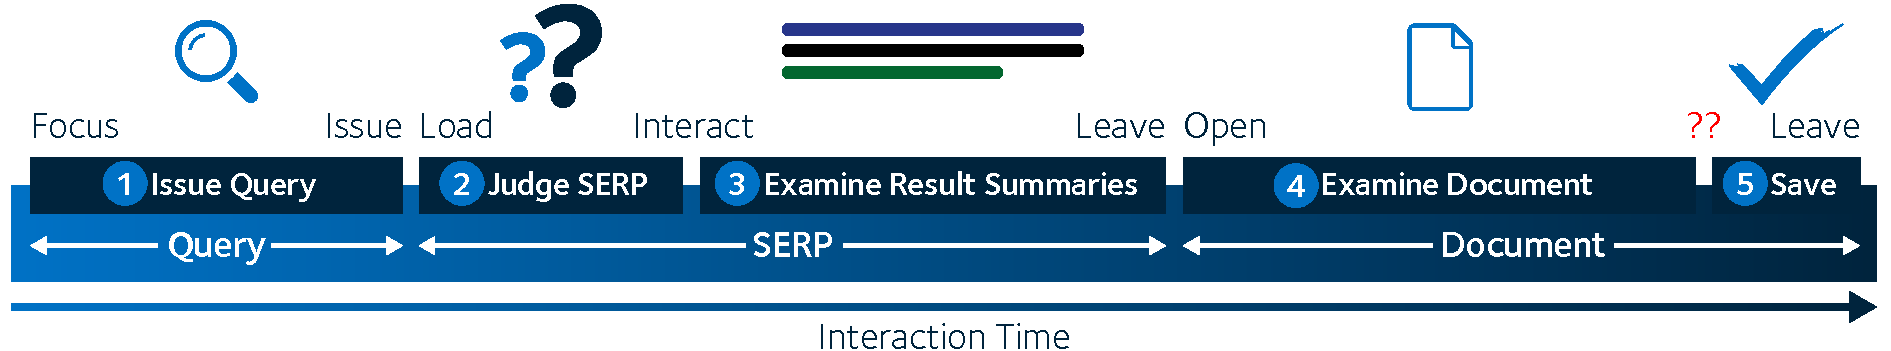
\includegraphics{figures/ch6-costs.pdf}}
    \caption[Interaction costs]{Illustration of the five interaction costs paid by searchers subscribing to the~\gls{acr:csm}. Each cost is shown with the start and end events, by which the costs were measured from the user study interaction logs. Time spent on individual components is shown in white. Refer to Section~\ref{sec:method:simulation:grounding:costs} for a detailed explanation of each interaction cost considered.}
    \label{fig:costs}
\end{figure}

The derived costs are averaged for each of the conditions and interfaces trialled in the studies reported in Chapters~\ref{chap:snippets} and~\ref{chap:diversity}. Refer to these chapters to tables of the actual costs used that were extracted from the corresponding interaction log data.

\blueboxheader{Fixed Interaction Costs}
All simulations of interaction discussed in this thesis rely upon the notion that all interaction costs are \emph{fixed} over each interface and condition trialled. That is, for example, no variation in the querying time between a simulated searcher exists who issues a query of one term versus a searcher who issues a query consisting of three terms. This decision was taken primarily to reduce the complexity of our simulations. By including dynamic interaction costs, this would have made the simulations themselves -- and the subsequent comparisons -- much more complex. Previous work such as time-biased gain~\citep{smucker2012tbg} has however shown that estimations of dynamic interaction costs can be made.

\subsubsection{Query Generation Strategies}\label{sec:method:simulation:grounding:querying}
The generation of queries is an important aspect of any simulation of interaction. Starting from the simplistic~\gls{acr:trec}-style searcher model where a single query is issued, numerous studies have focused upon the issue of query generation, and how one can generation a series of pseudo-realistic queries. We highlight some of these prior works in Section~\ref{sec:ir_background:user:simulation}.

In this thesis, we consider a number of different \emph{querying strategies} as proposed by~\cite{keskustalo2009querying} and~\cite{baskaya2013behavioural_factors} in order to generate queries for our simulations of interaction. These strategies are considered to be \emph{idealised, prototypical} approaches to query generation, being grounded from a prior user study examining the query behaviour of subjects.\footnote{Refer to~\cite{keskustalo2009querying} for further information on the user study undertaken.} Of the five strategies identified by the authors, we consider two in this thesis that were shown in simulations by~\cite{keskustalo2009querying} to yield the \emph{worst} and \emph{best} performance, but also shown to reflect actual searcher queries. The two querying strategies, identified as \blueboxbold{QS1} and \blueboxbold{QS3}, are briefly explained below. We also provide an illustration of the two strategies in Figure~\ref{fig:querying}, where $Q_n$ denotes query $n$ within a search session, and $t_n$ denotes query term $n$ from a list of terms available to formulate queries.

\begin{figure}[t!]
    \centering
    \resizebox{1\hsize}{!}{
    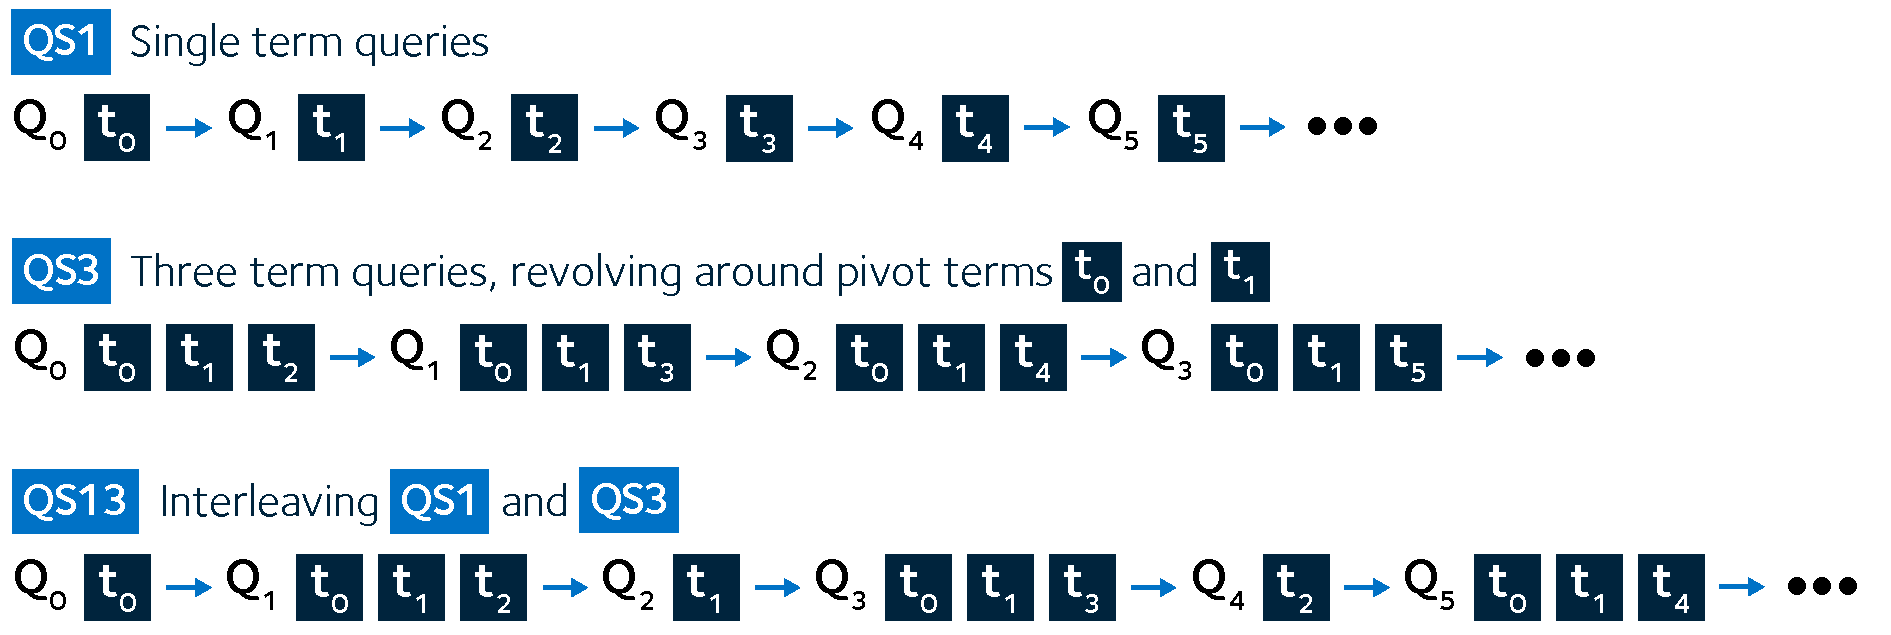
\includegraphics{figures/ch6-querying.pdf}}
    \caption[Querying strategies example]{Extensive examples of the four querying strategies used in this thesis, \blueboxbold{QS1}, \blueboxbold{QS3}, and \blueboxbold{QS13}. Queries are denoted by \emph{Q\textsubscript{n}}, with individual terms denoted by \darkblueboxbold{t\textsubscript{n}}. In these examples, a total of six terms are used (from \darkblueboxbold{t\textsubscript{0}} to \darkblueboxbold{t\textsubscript{5}}). Queries are separated by arrows (~
\includegraphics[height=\fontcharht\font`\d]{figures/src/arrow-blue-right.pdf}).}
    \label{fig:querying}
\end{figure}

\begin{itemize}
    \item{\blueboxbold{QS1 (Single Term)} This querying strategy generates a series of \emph{single term queries.}}
    \item{\blueboxbold{QS3 (Three Term)} This second querying strategy generates queries with two \emph{pivot} terms, and one other term. The first two terms therefore remain constant, with the third term changing for each subsequent query.}
\end{itemize}

These queries are relatively short, and are considered realistic in the sense that queries issued in real-life web search sessions consist three terms on average~\citep{keskustalo2009querying}.

With these two querying strategies in mind, we then combined them together to \emph{interleave} both of the querying strategies defined above. This therefore yields a further querying strategy, \blueboxbold{QS13}.

\begin{itemize}
    \item{\blueboxbold{QS13 (Interleaved)} With this querying strategy, queries from both \blueboxbold{QS1} and \blueboxbold{QS3} are generated, and subsequently interleaved between each other, starting with the first query from \blueboxbold{QS1}.}
\end{itemize}

Refer to Figure~\ref{fig:querying} for an example of how this querying strategy works. This querying strategy allowed us to test the \emph{robustness} of each result summary stopping strategy.~\cite{keskustalo2009querying} highlighted that \blueboxbold{QS1} yielded relatively poor performance compared to \blueboxbold{QS3}. It therefore follows that a searcher, when issuing a query generated by \blueboxbold{QS1}, will observe that the results presented are of poor quality, and thus stop at a shallow depth when compared to examining results of queries issued by \blueboxbold{QS3}. Examining many results from a poor query is by and large a waste of the searcher's time, so robustness of result summary stopping strategies can be checked to see if queries generated by \blueboxbold{QS1} are abandoned earlier than those generated by \blueboxbold{QS3}.

\blueboxheader{Reported Querying Strategy}
In this section, we introduced three different querying strategies -- two underlying querying strategies from the work by~\cite{keskustalo2009querying}, and one based upon this prior work. The latter allows us to test the robustness of various simulation configurations, and thus a majority of the work in this thesis reports on simulations that ran \blueboxbold{QS13} only. To examine the realism of different simulation configurations, we also \emph{replayed} queries issued by the real-world subjects of the two user studies reported in this thesis -- refer to Section~\ref{sec:method:simulation:runs:comparison} for further information.

\blueboxheader{Term List Generation}
Given the querying strategies, how did we then generate the ranked list of terms to be used, shown as \darkblueboxbold{t\textsubscript{0}} to \darkblueboxbold{t\textsubscript{5}} in Figure~\ref{fig:querying}? For all simulations in this thesis, all terms were derived from the given~\gls{acr:trec} topic title and description. For all queries, stopwords were removed as per the stopword list defined by~\cite{fox1992stopwords}.

For \blueboxbold{QS1}, we combined the title and description terms together and creating a \emph{Maximum Likelihood Estimate (MLE)} language model, allowing us to create a probability distribution for the likelihood of a term to appear in a topic description, i.e. $p(term|topic)$. A list of single term queries were then ranked in descending order by this probability to yield the set of queries we would use for \darkblueboxbold{t\textsubscript{0}}, \darkblueboxbold{t\textsubscript{1}} and so on.

A similar approach was used for \blueboxbold{QS3}. The same MLE approach was used to rank the title and description terms separately, creating two separate rankings of terms. For the \emph{pivot terms} -- the two terms that are consistently used as the first two terms of each \blueboxbold{QS3} query -- all possible two term title terms were used, with the highest joint probability being selected as terms \darkblueboxbold{t\textsubscript{0}} and \darkblueboxbold{t\textsubscript{1}}. Single terms from the topic description were then used as per \blueboxbold{QS1}, with the descending probability ordering used to then determine the third query term.

\subsubsection{Summary and Document Decision Making}\label{sec:method:simulation:grounding:judgements}
As discussed earlier in Section~\ref{sec:method:simulation}, our simulations were stochastic in nature with decisions pertaining to the attractiveness of a result summary \emph{(should I click this link and examine it further?)} and the relevancy of a document to the given information need \emph{(should I save this document?)} determined through a series of different \emph{interaction probabilities.} Chapters~\ref{chap:snippets} and~\ref{chap:diversity} present the interaction probabilities used within the simulations. In this section, we describe the approached used to derive them.

Like in previous studies considering the simulation of interaction -- such as those by~\cite{yilmaz2010browsing_utility} and~\cite{baskaya2013behavioural_factors} for instance -- result summary and document decision making revolve around two key probabilities:

\begin{itemize}
    \item{the probability \blueboxbold{P(C)} of considering a given result summary on a~\gls{acr:serp} to be sufficiently attractive to \emph{`click'} and load the associated document; and}
    \item{the probability \blueboxbold{P(S)} of determining the document to be relevant to the given information need after examination, and thus \emph{saving} it.}
\end{itemize}

These are considered separately as the action of requesting a document from clicking on the associated result summary does not necessarily mean that the document \emph{is} relevant; merely, it means it appears attractive enough to examine in more detail~\citep{turpin2009summaries}. The above probabilities are broken down further with regards to~\gls{acr:trec} relevance. This entails examination of the~\gls{acr:trec} relevance judgements to determine whether the result summary and/or document being clicked and/or saved was considered to be relevant to the given topic by the~\gls{acr:trec} assessors. As such, $P(C)$ and $P(S)$ can be split further, such that we can then determine:

\begin{itemize}
    \item{the probability that a result summary clicked is~\gls{acr:trec} relevant \blueboxbold{P(C|R)} or not \blueboxbold{P(C|N)}; and}
    \item{the probability that a document saved is~\gls{acr:trec} relevant \blueboxbold{P(S|R)} or not \blueboxbold{P(S|N)}.}
\end{itemize}

Taking these explanations, we could then take the interaction logs from the two user studies, split the interactions by the interface or condition that probabilities were to be derived for, and summate different measures -- as shown by the equation for calculating $P(C)$, where

\begin{equation}
    P(C) = \frac{|clicked_{Rel}| + |clicked_{\neg Rel}|}{examined}
\end{equation}

and $P(S)$, where

\begin{equation}
    P(S) = \frac{|saved_{Rel}| + | saved_{\neg Rel} |}{examined}.
\end{equation}

In the above equations, $Rel$ denotes the count for~\gls{acr:trec} relevant items, with $\neg Rel$ representing items that were not~\gls{acr:trec} relevant. Finally, $|clicked|$ represents the number of result summaries that were clicked (deemed attractive enough to examine further), $examined$ denotes the greatest depth at which searchers clicked on a result summary, with $|saved|$ denoting the number of documents that were identified as relevant, and subsequently \emph{saved.}

To compute probabilities concerning~\gls{acr:trec} relevance only, $P(C|R)$ and $P(S|R)$) were defined as $P(C|R) = \frac{|clicked_{Rel}|}{|examined_{Rel}|}$ and $P(S|R) = \frac{|saved_{Rel}|}{|examined_{Rel}|}$. These definitions are the same as the above, sans the non-relevant, or $\neg Rel$ values. Conversely, $P(C|N)$ and $P(C|R)$ were defined as $P(C|N) = \frac{|clicked_{\neg Rel}|}{examined_{\neg Rel}}$ and $P(S|N) = \frac{|saved_{\neg Rel}|}{examined_{\neg Rel}}$ -- this time, without the relevant judgements included.

\blueboxheader{Monte-Carlo Simulations}
The stochastic approach to modelling interactions provides a simple means of operationalising the components of the simulation that attempt to judge the attractiveness and relevancy of result summaries and documents, respectively.\footnote{A stochastic approach is not the only way the model such a process. For example,~\cite{maxwell2016agents} considered a \emph{deterministic} approach. A classifier was trained that then allowed a \emph{simulated agent} to deterministically decide the attractiveness of a result summary, for example.}

However, such an approach is not without limitation. By their vary nature, a stochastic simulation based upon random probabilities will require a large number of different trials to be executed from which an \emph{average} can be computed. Each trial will potentially result in a different outcome, as illustrated in Figure~\ref{fig:multiple_runs}. With a probability of clicking document \texttt{APW20000511.0185} set to $0.6\overline{6}$, there is a $66.6\overline{6}\%$ chance that the document would be clicked in each run, resulting in different outcomes across trials.

\begin{figure}[t!]
    \centering
    \vspace{4mm}
    \resizebox{1\hsize}{!}{
    
\includegraphics{figures/ch6-multiple_runs.pdf}}
    \caption[The problem of stochastic judgements]{An example of the same~\gls{acr:trec} relevant document being judged differently across multiple trials. This can have a negative effect upon simulation runs, yielding dubious results.}
    \label{fig:multiple_runs}
\end{figure}

Different outcomes can subsequently lead to a huge variance between different trials, which in turn leads to a requirement of running a larger number of trials, or \emph{Monte-Carlo style simulations}~\citep{benov2016manhattan}. In turn, this leads to a huge increase in the amount of time required to execute all simulations, as well as the computational power required.

\begin{table}[t!]
    \caption[Example of re-rolled judgements]{A visual example of how the use of pre-rolled judgements (right) performs when compared without (left). The top five rankings (from \emph{D\textsubscript{1}} to \emph{D\textsubscript{5}}) across four examples are shown. On the left are two simulated searcher configurations that do not use pre-rolled judgements. On the right, the same configurations are shown with pre-rolled judgements. Notice that for the examples with pre-rolled judgements, the same judgements are provided across configurations. On the left, this is not the case – indeed, this phenomenon can have an undue influence upon the behaviour of a simulated searcher, such as affecting their stopping behaviour. This is illustrated below, with the stopping depth for \dualbluebox{SS2}{@2} being affected (where stopping depths are highlighted in red).}
    \label{tbl:precomputed_judgements}
    \renewcommand{\arraystretch}{1.8}
    \begin{center}
    \vspace*{-2mm}
    \begin{tabulary}{\textwidth}{D{1.52cm}@{\CS}D{1.52cm}@{\CS}D{1.52cm}@{\CS}D{1.52cm}@{\CSDOUBLE}D{1.52cm}@{\CS}D{1.52cm}@{\CS}D{1.52cm}@{\CS}D{1.52cm}}
    
    \RS \multicolumn{4}{@{\hskip 6pt}c@{\CSDOUBLE}}{\textbf{Without pre-rolled (non-comparable)}} & \multicolumn{4}{@{\hskip 0pt}c}{\textbf{With pre-rolled (comparable)}}\\
    
    \RS \multicolumn{2}{@{\hskip 6pt}c@{\CS}}{\lbluecell \textbf{SS1@5}} & \multicolumn{2}{@{\hskip 0pt}c@{\CSDOUBLE}}{\lbluecell \textbf{SS2@2}} & \multicolumn{2}{@{\hskip 0pt}c@{\CS}}{\lbluecell \textbf{SS1@5}} & \multicolumn{2}{@{\hskip 0pt}c@{\hskip 6pt}}{\lbluecell \textbf{SS2@2}}\\
    
    \RS \lbluecell\textbf{D\textsubscript{1}} & \cell R & \lbluecell\textbf{D\textsubscript{1}} & \cell N & \lbluecell\textbf{D\textsubscript{1}} & \cell R & \lbluecell\textbf{D\textsubscript{1}} & \cell R\\
    \RS \lbluecell\textbf{D\textsubscript{2}} & \cell N & \lbluecell\textbf{D\textsubscript{2}} & \cell R & \lbluecell\textbf{D\textsubscript{2}} & \cell R & \lbluecell\textbf{D\textsubscript{2}} & \cell R\\
    \RS \lbluecell\textbf{D\textsubscript{3}} & \cell N & \lbluecell\textbf{D\textsubscript{3}} & \lredcell N & \lbluecell\textbf{D\textsubscript{3}} & \cell N & \lbluecell\textbf{D\textsubscript{3}} & \cell N\\
    \RS \lbluecell\textbf{D\textsubscript{4}} & \cell R & \lbluecell\textbf{D\textsubscript{4}} & \cell R & \lbluecell\textbf{D\textsubscript{4}} & \cell R & \lbluecell\textbf{D\textsubscript{4}} & \cell R\\
    \RS \lbluecell\textbf{D\textsubscript{5}} & \lredcell R & \lbluecell\textbf{D\textsubscript{5}} & \cell R & \lbluecell\textbf{D\textsubscript{5}} & \lredcell N & \lbluecell\textbf{D\textsubscript{5}} & \lredcell N\\
\end{tabulary}
\vspace*{-3mm}
\end{center}
\end{table}

\blueboxheader{Pre-Rolled Judgements}
In Figure~\ref{fig:multiple_runs}, if the same document is judged differently between individual trials, then results from two different simulated searcher configurations are non-comparable. This is demonstrated in the left hand side of Table~\ref{tbl:precomputed_judgements}. With a given probability, a result summary can be judged to be attractive or not ($P(C)$). Without proper controls, these judgements will vary across trials, meaning that in Table~\ref{tbl:precomputed_judgements}, \dualbluebox{SS1}{@5} and \dualbluebox{SS2}{@2} are non-comparable (refer to Section~\ref{sec:method:simulation:grounding:stopping} for more information on these configurations) because the judgements for the same ranked list of results differ. As these judgements change, this has influences the behaviour of the simulated searcher across the configurations.

In order to address this issue and permit for fair comparisons across simulated searcher configurations, and to allow for reproducible results, we used a series of \emph{pre-rolled} judgements that determined the attractiveness or relevancy of result summaries and documents respectively \emph{a priori.} For each document within the AQUAINT collection, we pre-computed outcomes for each individual document, storing them in \emph{action judgement files.} One related to the action of clicking on result summaries (i.e. $P(C)$), with the other related to saving documents (i.e. $P(S)$). These judgement files were then used by the summary and document decision maker component. All this component had to do was then perform a simple lookup for the corresponding document judgement for a given trial.

By pre-computing these judgements in advance, the same document would therefore be considered to be relevant in the same trial under a different configuration. This is demonstrated again in Table~\ref{tbl:precomputed_judgements}, this time on the right hand side. Across this example trial, judgements by the simulated searcher have been pre-rolled in advance, and thus the judgements for documents $D_1$ to $D_5$ are the same. As they are the same, this permits a fairer comparison between the different configurations, with the table again showing how the simulated searcher's behaviour varies.

It should also be noted that the generated pre-rolled judgements were seeded to allow for these files to be easily reproduced. This process was repeated 50 times, meaning that for every simulated searcher configuration, we ran a total of 50 trials in which result summaries could be considered attractive or not, and documents could be considered relevant or not. This subsequently means that for each comparison, all results reported later in this thesis are an average over the 50 trials.

\subsubsection{Computing Gain}\label{sec:method:simulation:grounding:gain}
As searchers examine information, they \emph{gain knowledge} that helps shape their mental model of the underlying information need~\citep{nickles1995judgment}. In the simulations reported in this thesis, gain is acquired when a simulated searcher, having examined a document, subsequently considers said document is relevant, and saves it. During post-hoc analysis, we then can compute how many documents were saved, and how many were saved and~\gls{acr:trec} relevant. This is determined by looking up the~\gls{acr:trec} relevancy judgements. Gain for the document is then simply computed as the relevancy judgement score from the~\gls{acr:trec} QRELs. Given that we utilised the~\gls{acr:trec} 2005 Robust Track~\citep{voorhees2005trec_book}, \emph{graded relevance judgements} are used. This value, when summated over all saved documents, is the~\glsfirst{acr:cg} score for a simulated trial. This is discussed in more detail in Section~\ref{sec:method:simulation:runs}.

\vspace*{-2mm}
\subsubsection{SERP Level Decision Making}\label{sec:method:simulation:grounding:serp}
Previously outlined in Section~\ref{sec:csm:stopping}, the~\gls{acr:csm} includes an additional~\gls{acr:serp} level stopping decision point. Motivated by the \emph{information scent}\footnote{To recap, we discuss the notion of information scent in Section~\ref{sec:stopping_background:theoretical:ift:patch}.} offered by a~\gls{acr:serp} (or \emph{patch}), this stopping point joins other established decision points, including result summary and session level stopping. The new decision point permits a searcher subscribing to the~\gls{acr:csm} to either \emph{enter} the~\gls{acr:serp} and begin examining result summaries in detail (if the~\gls{acr:serp}) appears to offer a good scent, or abandon the~\gls{acr:serp} if it appears to be poor, and thus save time.

For our simulated analyses of the user studies reported in Chapters~\ref{chap:snippets} and~\ref{chap:diversity}, the~\gls{acr:serp} level stopping decision point is not considered. In other words, a simulated searcher will \emph{always} examine a given~\gls{acr:serp} for content in detail -- labelled \blueboxbold{Always} in this thesis. This acts as our baseline for the~\gls{acr:serp} level stopping decision point. This decision was taken to simplify our results and to provide greater emphasis upon how the different snippet level stopping strategies (as discussed below in Section~\ref{sec:method:simulation:grounding:stopping}) affect searcher behaviour and performance.

Our final contributory chapter, Chapter~\ref{chap:serp}, provides empirical results when varying the ways in which the new~\gls{acr:serp} level stopping decision point is considered. This chapter also provides a detailed explanation as to how we operationalised this new stopping decision point, outlined in Section~\ref{sec:serp:method:serp_dp}.

\subsubsection{Result Summary Level Stopping Strategies}\label{sec:method:simulation:grounding:stopping}
In Chapter~\ref{chap:strategies}, we outlined twelve stopping strategies that had been operationalised from various stopping heuristics and an~\gls{acr:ir}-based evaluation measure. In this section, we once again enumerate each of the different stopping strategies, discussing what \emph{stopping threshold values} that we trialled for each.

For several of the stopping strategies, threshold values need to be approximated from real-world interaction data to provide grounding. An example of such a threshold is the~\gls{acr:rbp} patience parameter, as we discussed in Section~\ref{sec:ir_background:evaluation:system:rbp}. As such, some of the threshold value ranges were approximated from the user study interaction data in Chapter~\ref{chap:snippets}, and used in all simulation experimentation for consistency. The values that we ascertained were of most interest as they offer close approximations to how real-world searchers actually behaved.

Below, we begin our discussion of each of the different stopping strategies, outlining the parameter thresholds used.

\begin{itemize}
    \item{\blueboxbold{SS1-FIX} For our fixed depth stopping strategy, we trialled a range of values, where $x_1$ was set from $1$ to $10$ in steps of $1$, and then $15$ to $24$ in steps of $3$. This resulted in $14$ separate parameter threshold configurations, with enough values such that a searcher would comfortably reach the time limits imposed in the study detailed in Chapter~\ref{chap:snippets}.}
    
    \item{\blueboxbold{SS2-NT} and \blueboxbold{SS3-NC} The same range of values were used for threshold values $x_2$ and $x_3$. These stopping strategies focused upon a searcher's tolerance to non-relevance, as discussed in Section~\ref{sec:strategies:frus_disg:frustration}.}
\end{itemize}

Next, we enumerate the stopping strategy considering the \emph{satiation}~\citep{simon1955satiation} of a searcher.

\begin{itemize}
    \item{\blueboxbold{SS4-SAT} Concerning the number of documents that a searcher should save before being satisfied, we examined a range of values for $x_4$, from $1$ to $10$ in steps of $1$.}
\end{itemize}

Our combination heuristic then combines the frustration and satisfaction heuristics together. However, two frustration stopping strategies exist -- \blueboxbold{SS2-NT} and \blueboxbold{SS3-NC}. To reduce the complexity of the simulations -- and to corroborate with empirical evidence suggesting that this was the better performing strategy (refer to~\cite{maxwell2015stopping_strategies}), \blueboxbold{SS2-NT} is considered to be the non-relevant component of the combination strategy.

\begin{itemize}
    \item{\blueboxbold{SS5-COMB} We utilised the stopping threshold values defined for $x_2$ and $x_4$ above. These were for the frustration component \blueboxbold{SS2-NT} and \blueboxbold{SS4-SAT} respectively.}
\end{itemize}

Next, we consider the two stopping strategies that focus upon the difference threshold heuristic~\citep{nickles1995judgment}, where searchers would abandon a set of results if the summaries provided did not yield any new information.

\begin{itemize}
    \item{\blueboxbold{SS6-DT} Considering the term overlap difference between a result summary and prior summaries, a range of values from $0.0$ to $1.0$ in steps of $0.05$. This was to explore the entire range of possible values. The smaller the threshold, the less similar the content of the new result summary to those previously examined.}
    
    \item{\blueboxbold{SS7-DKL} Using~\gls{glos:kl}, a range of values for $x_7$ were trialled, from $3.0$ to $8.0$ in steps of $0.5$. A small-scale pilot study examining this stopping strategy over the AQUAINT index showed that a majority of values fell within this range.}
\end{itemize}

For both \stoppingstratboxsingular{SS6-DT} and \stoppingstratboxsingular{SS7-DKL}, we considered both the \emph{per-query difference} and the \emph{per-session difference.} For the per-query variant, previously observed result summaries consisted of the first result summary, thus meaning that the simulated searcher would always consider at least two result summaries before deciding to stop. For the per-session variant, all previously observed result summaries over the entire search session (i.e. including those from previous queries) were used. In a pilot study, as reported by~\cite{maxwell2015initial_stopping}, we consider in this thesis the per-query variants only. These offered better performance than their per-session variants.

Next we consider the stopping strategy based upon a searcher's optimal foraging behaviour. This concerned computing a searcher's \emph{average rate of gain.} To determine the rate of gain at a given result summary at rank $i$, we first computed the~\gls{acr:dcg} (discussed in Section~\ref{sec:ir_background:evaluation:system:cg}) received from the observed documents, up to the point in the ranked list at position $i$. We then divided $g$ by the total time taken, yielding $i * t_d + t_q$, where $i$ represented the rank, $t_d$ was the time required to examine a document, and $t_q$ was the time required to issue a query.

\begin{itemize}
    \item{\blueboxbold{SS8-IFT} Computing the searcher's average rate of gain as defined above, we considered a gain threshold ($x_8$) from $0.002$ to $0.03$ in steps of $0.002$. A minimum of two result summaries were examined before calculating the average rate of gain ($y_8=2$).}
\end{itemize}

The estimate computed was very dependent upon the first document in the ranked list. For example, if judged to be non-relevant, the searcher would gain $0$ -- meaning that the searcher would then immediately stop when $x_8 > 0$. To counter this, we also considered an additional parameter that specified how many result summaries the searcher should \emph{always} examine before making a decision based upon the rate of gain experienced.\footnote{This second parameter $y_8$ was set to $2$ for all experiments utilising \blueboxbold{SS8-IFT}. A pilot study by~\cite{maxwell2015stopping_strategies} found that a value of $2$ proved to be far less sensitive to non-relevant items, and resulted in better performance by the searcher.} This would essentially mean that a searcher employing \blueboxbold{SS8-IFT} would look at a minimum of $y_8$ result summaries, and from there begin to make decisions as to the whether they should continue.

Next, we consider the time-based stopping strategies as outlined in Section~\ref{sec:strategies:time}. These consider the total time spent examining a~\gls{acr:serp} and its associated documents, and the time since last identifying a relevant document.

\begin{itemize}
    \item{\blueboxbold{SS9-TIME} Considering the total amount of time spent on a~\gls{acr:serp} and linked documents, we considered for this \emph{total time} stopping strategy values for $x_9$ from $30$ to $150$ seconds in steps of $30$ seconds.}
    
    \item{\blueboxbold{SS10-RELTIME} Stopping (or \emph{giving up}~\citep{krebs1974leave_after_rule}) after $x_{10}$ seconds have elapsed since saving a relevant document (or the start of the search session if no documents have been saved), we consider for this stopping strategy a smaller range of values, from $10$ to $50$ seconds in steps of $10$ seconds.}
\end{itemize}

The parameter threshold values for $x_9$ and $x_{10}$ were grounded using interaction data derived from the user study discussed in Chapter~\ref{chap:snippets}. For $x_9$, the mean time spent interacting on a~\gls{acr:serp} and its documents was computed at approximately $90$ seconds -- a $60$ second decrease and increase were selected for the lower and upper bounds respectively. Likewise, a relevant document was on average identified approximately every $30$ seconds. As such, this provides motivation behind selecting the range of values chosen for $x_{10}$.

The second combination rule, based upon the combination heuristic proposed by~\cite{mcnair1982gut_mvt}, considers that a searcher decides whether a given~\gls{acr:serp} is of a high or low scent. Depending upon the scent observed, a different stopping strategy will be employed.

\begin{itemize}
    \item{\blueboxbold{SS11-COMB} For a high scented~\gls{acr:serp}, a searcher will employ the satisfaction stopping heuristic, \blueboxbold{SS4-SAT}. The give-up time-based strategy \blueboxbold{SS10-RELTIME} is employed if the scent is low. Parameter threshold values are identical to those defined for $x_4$ and $x_{10}$ above.}
\end{itemize}

Every possible combination of the values selected for $x_4$ and $x_{10}$ were trialled. To determine the scent of a given set of ranked results, we considered the first ranked result, or $P@1$. If~\gls{acr:trec} relevant, the results were assumed to provide a high scent, or a low scent if the document at rank one was not relevant.

The twelfth result summary level stopping strategy was based upon~\gls{acr:rbp}. Once again, the patience parameter was grounded from the user study outlined in Chapter~\ref{chap:snippets}.

\begin{itemize}
    \item{\blueboxbold{SS12-RBP} Given a fitted patience parameter of $0.9087$, we trialled a range of values around this area, from $0.8$ to $0.95$ in steps of $0.05$. We also trialled $0.99$ and $0.9087$.}
\end{itemize}

To estimate the patience parameter, we assumed that the patience of a searcher could be determined by considering the depths at which documents were clicked, as per~\gls{acr:rbp}. The deeper the searcher went down a list of ranked results, the more patient they were considered to be. For every query issued, we determined whether the document at each rank of the corresponding set of results was clicked or not, as shown in step~\raisebox{-.2\height}{
\includegraphics[height=5mm]{figures/ch2-point1.pdf}} below.

\begin{figure}[h]
    \centering
    \vspace{4mm}
    \resizebox{1\hsize}{!}{
    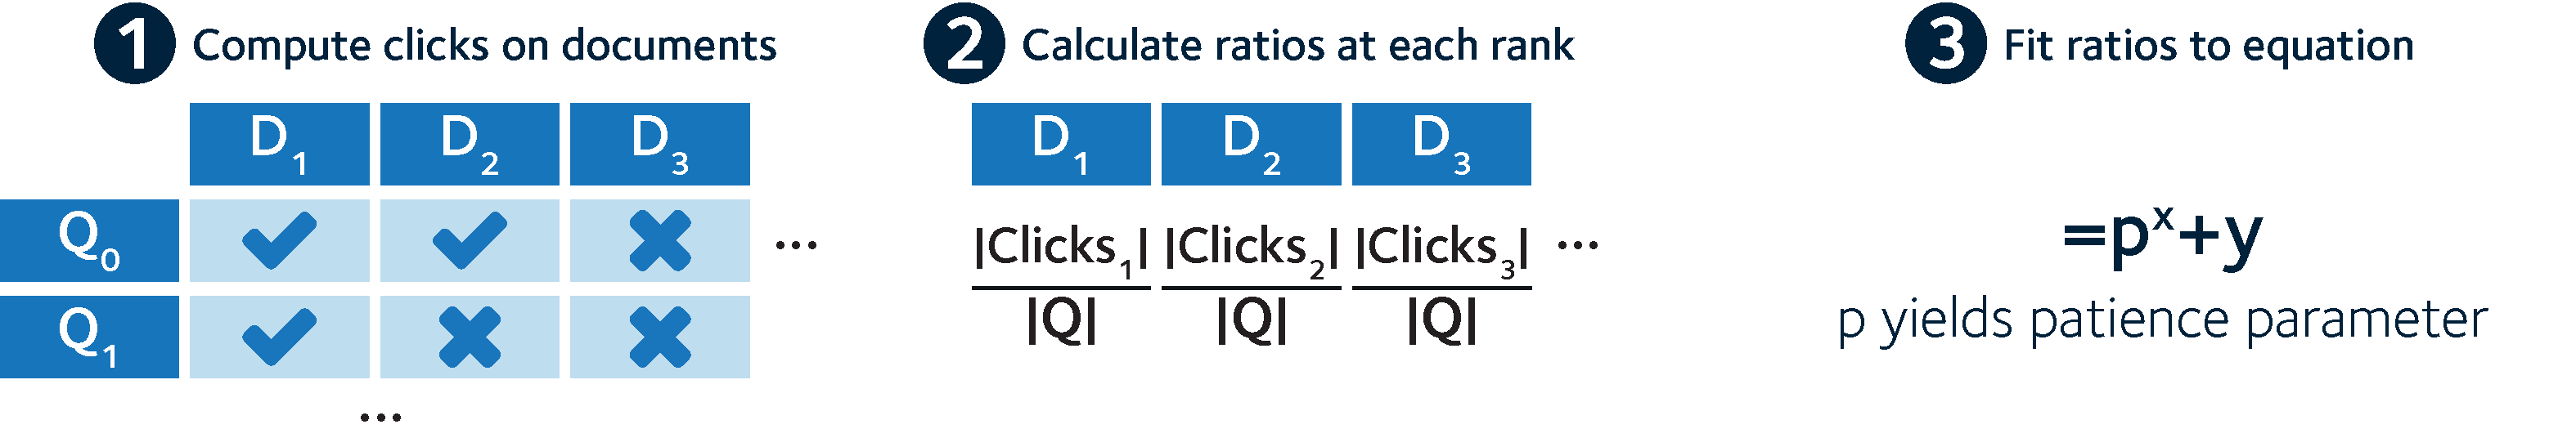
\includegraphics{figures/ch6-rbp.pdf}}
    \label{fig:rbp_patience}
    \vspace{-5mm}
\end{figure}

For each rank, we could then compute the ratio of clicks at each rank, across all queries, as demonstrated at step~\raisebox{-.2\height}{
\includegraphics[height=5mm]{figures/ch2-point2.pdf}}. This yielded a decreasing ratio as the depth increased -- demonstrating that searchers we less likely to click on results at greater depths. Finally, $p(click@k) = p^k$ was fit to the data. This represents the probability of clicking on a result summary at rank $k$, with $p$ denoting the~\gls{acr:rbp} patience parameter. When fit, the yielded value was $p=0.9087$.

Given the descriptions for each of the twelve stopping strategies, we conclude this section with a summary table. Table~\ref{tbl:stopping_thresholds} lists each of the stopping strategies, along with the different threshold parameter values that were trialled for each.

\begin{table}[t!]
    \caption[Stopping strategies thresholds summary table]{Summary table of the twelve stopping strategies, along with each of the threshold parameter values trialled. Note that for \blueboxbold{SS5-COMB} and \blueboxbold{SS11-COMB}, thresholds from different stopping strategies are used for the respective components of each combination strategy.}
    \label{tbl:stopping_thresholds}
    \renewcommand{\arraystretch}{1.8}
    \begin{center}
    \vspace*{-2mm}
    \begin{tabulary}{\textwidth}{L{4cm}@{\CS}L{11.8cm}}
    
    \RS \lbluecell\textbf{Stopping Strategy} & \lbluecell\textbf{Threshold Parameter Values} \\
    
    \RS \cell\textbf{SS1-FIX} & \cell x\textsubscript{1} = [1, 2, 3, ..., 8, 9, 10, 15, 18, 21, 24] \\
    \RS \cell\textbf{SS2-NT} & \cell x\textsubscript{2} = [1, 2, 3, ..., 8, 9, 10, 15, 18, 21, 24] \\
    \RS \cell\textbf{SS3-NC} & \cell x\textsubscript{3} = [1, 2, 3, ..., 8, 9, 10, 15, 18, 21, 24] \\
    \RS \cell\textbf{SS4-SAT} & \cell x\textsubscript{4} = [1, 2, 3, ..., 8, 9, 10] \\
    \RS \cell\textbf{SS5-COMB} & \cell x\textsubscript{2} = [1, 2, 3, ..., 8, 9, 10, 15, 18, 21, 24] \textbf{(SS2-NT)} \\
    & \cell x\textsubscript{4} = [1, 2, 3, ..., 8, 9, 10] \textbf{(SS4-SAT)} \\
    \RS \cell\textbf{SS6-DT} & \cell x\textsubscript{6} = [0.0, 0.05, 0.10, ..., 0.90, 0.95, 1.00] \\
    \RS \cell\textbf{SS7-DKL} & \cell x\textsubscript{7} = [3.0, 3.5, 4.0, ..., 7.0, 7.5, 8.0] \\
    \RS \cell\textbf{SS8-IFT} & \cell x\textsubscript{8} = [0.002, 0.004, 0.006, ..., 0.026, 0.028, 0.03] \\
    & \cell y\textsubscript{8} = 2 \\
    \RS \cell\textbf{SS9-TIME} & \cell x\textsubscript{9} = [30, 60, 90, 120, 150] \\
    \RS \cell\textbf{SS10-RELTIME} & \cell x\textsubscript{10} = [10, 20, 30, 40, 50] \\
    \RS \cell\textbf{SS11-COMB} & \cell x\textsubscript{4} = [1, 2, 3, ..., 8, 9, 10] \textbf{(SS4-SAT)} \\
    & \cell x\textsubscript{10} = [10, 20, 30, 40, 50] \textbf{(SS10-RELTIME)} \\
    \RS \cell\textbf{SS12-RBP} & \cell x\textsubscript{12} = [0.80, 0.85, 0.90, 0.9087, 0.95, 0.99] \\
    
\end{tabulary}
\vspace*{-3mm}
\end{center}
\end{table}

\subsubsection{Simulated Searcher Constraints and Goals}\label{sec:method:simulation:grounding:constraints}
Like in the corresponding user studies, we imposed different constraints upon the simulated searchers to keep the comparisons as fair as possible. For example, in Chapter~\ref{chap:snippets} a session time constraint was imposed. In Chapter~\ref{chap:diversity}, no time limit was imposed, but subjects were instead tasked to find four relevant documents under different search tasks. These constraints and goals are discussed in depth in the relevant chapter.

\subsection{Simulation Runs and Evaluation}\label{sec:method:simulation:runs}
Having now discussed how all of the various components of the~\gls{acr:csm} and the \simiir~framework were instantiated for our simulations, we now move onto a discussion of how we actually ran the simulations -- and evaluated them.

With two research questions regarding the empirical work presented in this thesis, we designed and executed a set of simulations runs to address each of them.

\begin{itemize}
    \item{\darkblueboxbold{HL-RQ3a} \emph{Given the aforementioned operationalised stopping strategies, how well does each one perform?}}
    \item[]{To address this research question, we propose a series of \blueboxbold{performance runs} that allow us to determine the best overall level of performance that can be attained using a particular configuration of simulated searcher, via a number of \emph{what-if} scenarios\footnote{\emph{What-if} scenarios are discussed in Section~\ref{sec:ir_background:user:simulation}.}.}
    
    \item{\darkblueboxbold{HL-RQ3b} \emph{How closely do the operationalised stopping strategies compare to the actual stopping behaviours of real-world searchers?}}
    \item[]{To address this second research question, we also propose a series of \blueboxbold{comparison runs} that instead focus upon how closely different configurations of simulated searcher approximate the stopping behaviours of real-world searchers.}
\end{itemize}

These simulations fit within the wider experimental framework discussed in this chapter, illustrated in Figure~\ref{fig:sim_evaluation}. Within the figure, we can see the link between the user studies and the two sets of simulations (highlighted with \darkblueboxbold{dark blue} boxes) via the act of \emph{grounding.} The illustration also provides linkage between the simulations, and the two sets of analyses that are undertaken -- the performance analysis, addressing \darkblueboxbold{HL-RQ3a}, and the behaviour comparison analysis that addressing \darkblueboxbold{HL-RQ3b}. The performance analysis is an examination of the hundreds of different possible simulation configurations, allowing us to explore how performance varies through what-if simulations. In all, this process is \textbf{\color{dmax_red} repeated twice}, once per user study (refer to Chapters~\ref{chap:snippets} and~\ref{chap:diversity}), as shown in the illustration. We discuss the two different sets of simulations that address research questions \darkblueboxbold{HL-RQ3a} and \darkblueboxbold{HL-RQ3b} in Sections~\ref{sec:method:simulation:runs:performance} and~\ref{sec:method:simulation:runs:comparison} respectively.

\begin{figure}[t!]
    \centering
    \resizebox{1\hsize}{!}{
    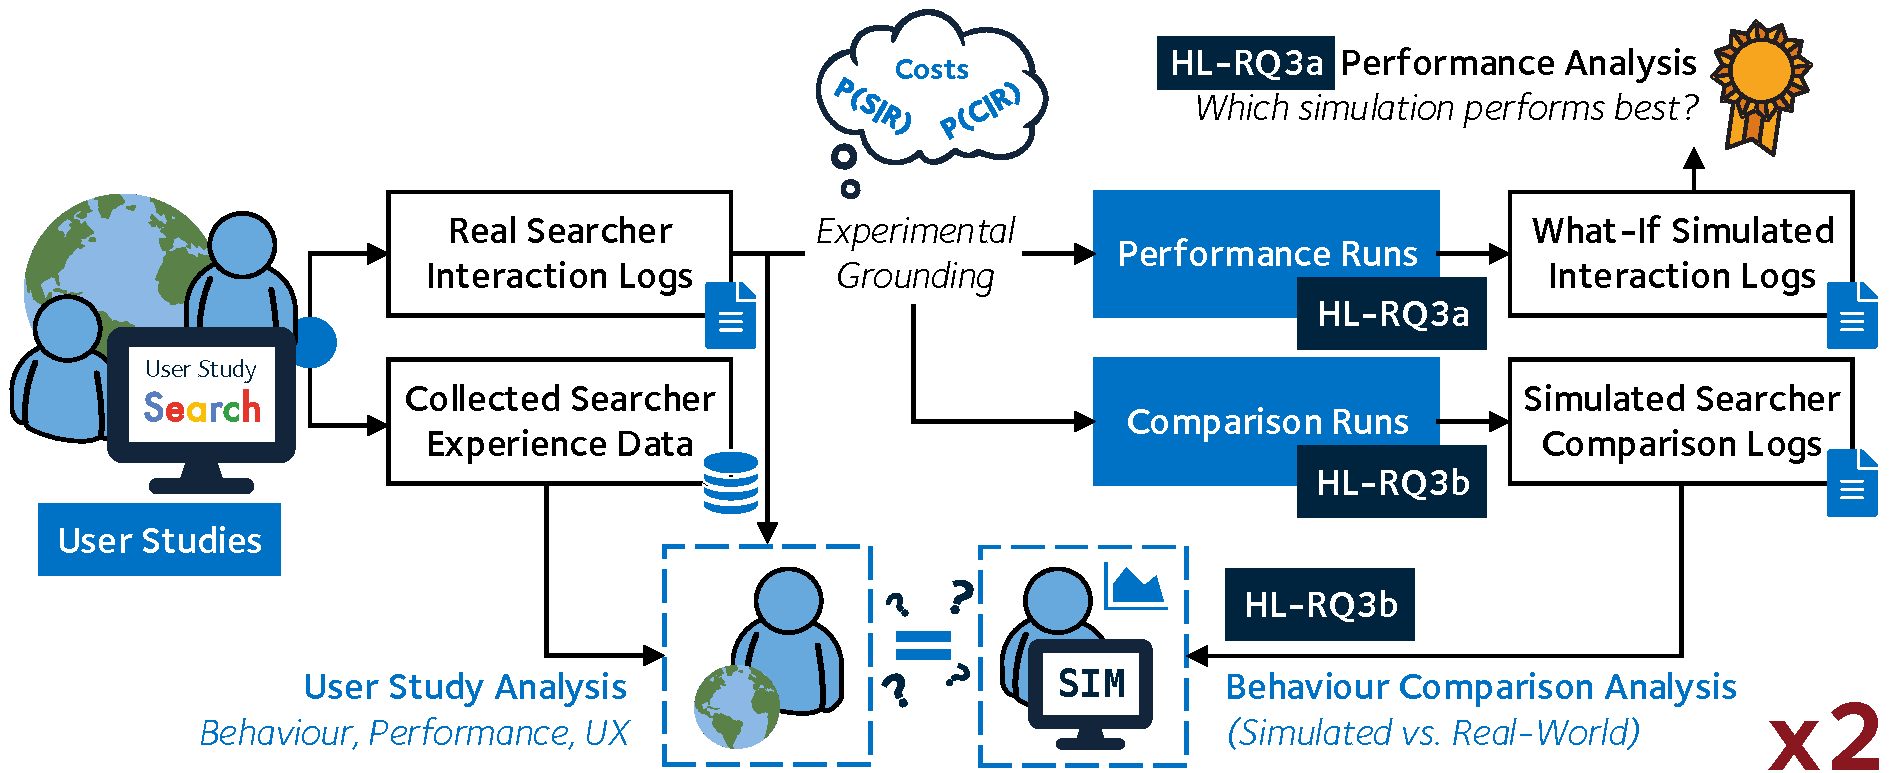
\includegraphics{figures/ch6-sim_evaluation.pdf}}
    \caption[Empirical evaluation framework]{How the two sets of simulations, represented as dark blue boxes, fit within the wider experimentation framework as discussed in this chapter. The illustration also shows what components address the two high level research questions, \darkblueboxbold{HL-RQ3a} and \darkblueboxbold{HL-RQ3b}.}
    \label{fig:sim_evaluation}
\end{figure}

\subsubsection{Performance Runs}\label{sec:method:simulation:runs:performance}
Named as a series of \emph{what-if} simulations above, the performance runs instantiate the different components of the~\gls{acr:csm} and \simiir~framework as previously discussed throughout Section~\ref{sec:method:simulation:grounding}. Using the grounded interaction probabilities and costs, these simulations were trialled over the five selected topics of the~\gls{acr:trec} 2005 Robust Track~\citep{voorhees2006trec_robust} (as discussed in Section~\ref{sec:methodology:collection:topics}), with queries generated via the querying strategy outlined in Section~\ref{sec:method:simulation:grounding:querying}. All in all, this provided us with a wealth of simulated interaction data from which we could calculate a series of averages over the different trials experimented. As illustrated in the example figure below, we then computed the various performance measures (unless otherwise stated) over each simulated searcher configuration, taking an average over each of the five topics.

\begin{figure*}[h]
    \centering
    \resizebox{1\hsize}{!}{
    \vspace*{5mm}
    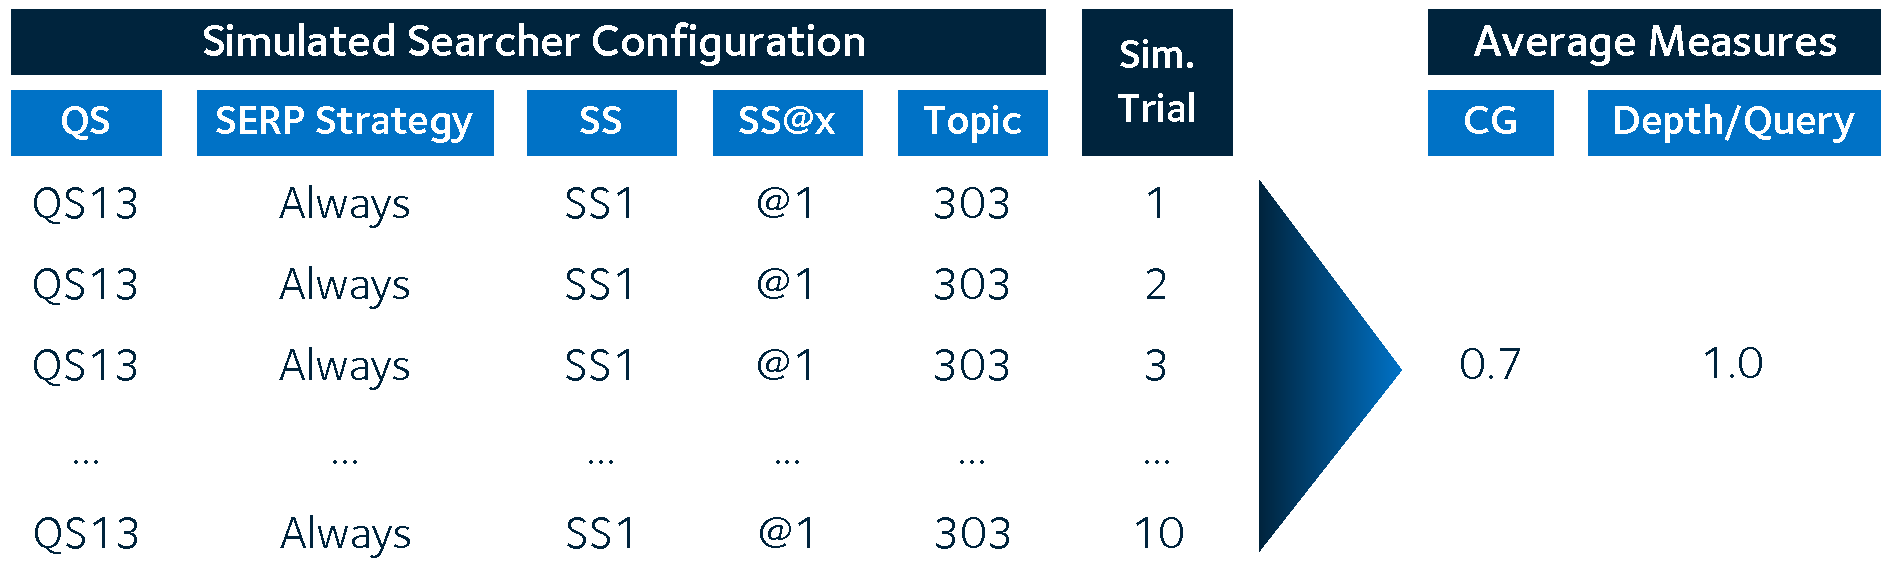
\includegraphics{figures/ch6-performance.pdf}}
    \vspace*{-6mm}
\end{figure*}

This example illustrates a single configuration of simulated searcher, using: querying strategy \blueboxbold{QS13}; the \blueboxbold{Always} (baseline)~\gls{acr:serp} examination strategy;
\stoppingstratbox{SS1-FIX}{1}; all while examining~\gls{acr:trec} topic \textnumero~367, all of which were in turn executed over 50 trials. This meant that over one individual simulated searcher configuration, a total of $500$ simulation trials were required. Section~\ref{sec:method:simulation:grounding:judgements} provides an explanation as to why these trials were required.

One criticism that can be levied upon this approach is the selection of \emph{five topics only.} With the~\gls{acr:trec} 2005 Robust Track containing a total of 50 topics, complete with~\gls{acr:trec} relevance judgements, why were only five selected? In Chapter~\ref{chap:diversity}, we report on a user study that employs \emph{aspectual retrieval}. For consistency, we employed the same index and topics. However, as we discuss in Section~\ref{sec:diversity:users:method:aspects} on page~\pageref{sec:diversity:users:method:aspects}, aspects are not part of the~\gls{acr:trec} 2005 Robust Track. Time was spent manually extracting aspects from all identified~\gls{acr:trec} relevant documents over the five selected topics -- the remaining 45 topics were not considered. For a fair comparison between different conditions and interfaces, we were therefore limited on the number of topics we could run. This is why a large number of runs were trialled -- a larger number of runs provided more data from which an average could be derived.

Given the name performance runs, we primarily examined the performance of each simulated searcher trialled. While examining the performance of queries (via the measures outlined previously in Section~\ref{sec:methodology:extracting:performance}), we also examined measures illustrated in the figure above: mean levels of~\gls{acr:cg}, and the mean \blueboxbold{depth per query (D/Q)}.

\gls{acr:cg} was discussed in passing in Section~\ref{sec:method:simulation:grounding:gain}. For our simulations, we consider the~\gls{acr:cg} as the amount of gain accrued over the \emph{course of a search session} -- which, by definition, can entail more than a single query. A more effective series of stopping strategies that are better at stopping a simulated searcher examining poor quality~\glsplural{acr:serp} in any great depth will therefore provide higher levels of~\gls{acr:cg}, but only if the queries issued offer good performance. Similarly, an effective~\gls{acr:serp} level stopping decision point implementation will stop the searcher from examining a poor~\gls{acr:serp} in the first instance, leaving more time to examine~\glsplural{acr:serp} that could potentially offer higher quality results.

The other major measure used in our performance measures was the depth per query. With this measure, performance is not measured, but rather the stopping behaviour of the simulated searchers. As shown in the illustration below, a fictional search session consists of three queries, $Q_0$, $Q_1$ and $Q_2$.

\begin{figure*}[h]
    \centering
    \resizebox{1\hsize}{!}{
    \vspace*{5mm}
    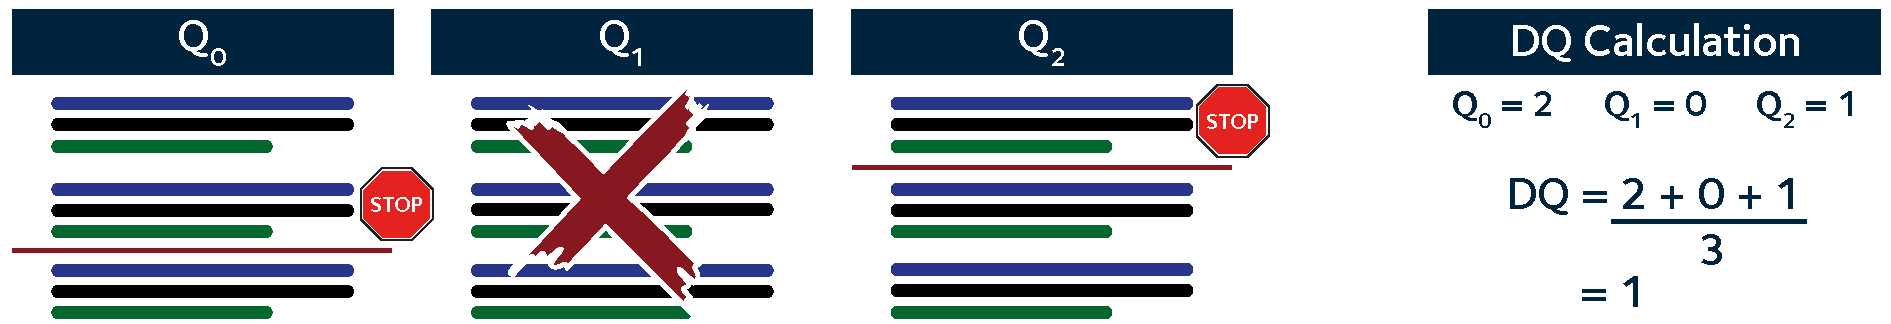
\includegraphics{figures/ch6-dq.pdf}}
    \vspace*{-6mm}
\end{figure*}

In the example, a simulated searcher examines to a depth of $2$ for $Q_0$, and a depth of $1$ for $Q_2$. The searcher does not even enter the associated~\gls{acr:serp} for $Q_1$, as the~\gls{acr:serp} level stopping decision point prevents the searcher from examining result summaries in detail. This resultant $D/Q$ for the search session is therefore $1$.

\subsubsection{Comparison Runs}\label{sec:method:simulation:runs:comparison}
Rather than focus upon the overall performance attained by simulated searchers under different scenarios, the second set of simulations we ran focused on comparing simulated searcher behaviours against their real-world counterparts. As such, the simulations for this set were run with minor differences in order to improve the ability for comparing the two populations of searchers -- both simulated and real-world. The first difference considered the querying component of the simulations:

\begin{itemize}
    \item{rather than considering the issuance of simulated queries via a querying strategy, we instead took the queries from the associated user study, and issued each one in turn. In effect, we \blueboxbold{replayed} all real-world queries issued (as discussed in Section~\ref{sec:method:simulation:grounding:querying}).}
\end{itemize}

Following the real-world queries, we improved the realism of our simulations yet further. Queries were extracted from those issued over each individual interface and condition trialled. This also provided us with the ability to perform a direct comparison on searcher behaviour at a query level, rather than across an entire search session. However, with only four topics trialled during the user studies, we considered only the \blueboxbold{four~\gls{acr:trec} topics}, omitting the practice topic (\textnumero~367). This was due to the fact that we only had real-world query data for the four topics trialled in the user studies. We once again ran a simulated searcher for each different configuration, over every query issued. A total of 50 trials were once again used, as explained in Section~\ref{sec:method:simulation:grounding:judgements}.

To perform our comparisons with the real-world searchers and simulated searchers, we used the \blueboxbold{Mean Squared Error (MSE)} to compute the difference between the two. For this, our calculations were performed between the click depth of the real-world searchers over each query, and taking the simulated click depths. Simulated click depths are defined as the depth of the last document that was considered attractive enough to examine on a given simulated~\gls{acr:serp}. Considering each of simulated searcher (i.e. a combination of~\gls{acr:serp} level stopping component and snippet level stopping strategy and threshold), we could then produce a table of click depths, as provided in the example below.

\begin{figure*}[h]
    \centering
    \resizebox{1\hsize}{!}{
    \vspace*{5mm}
    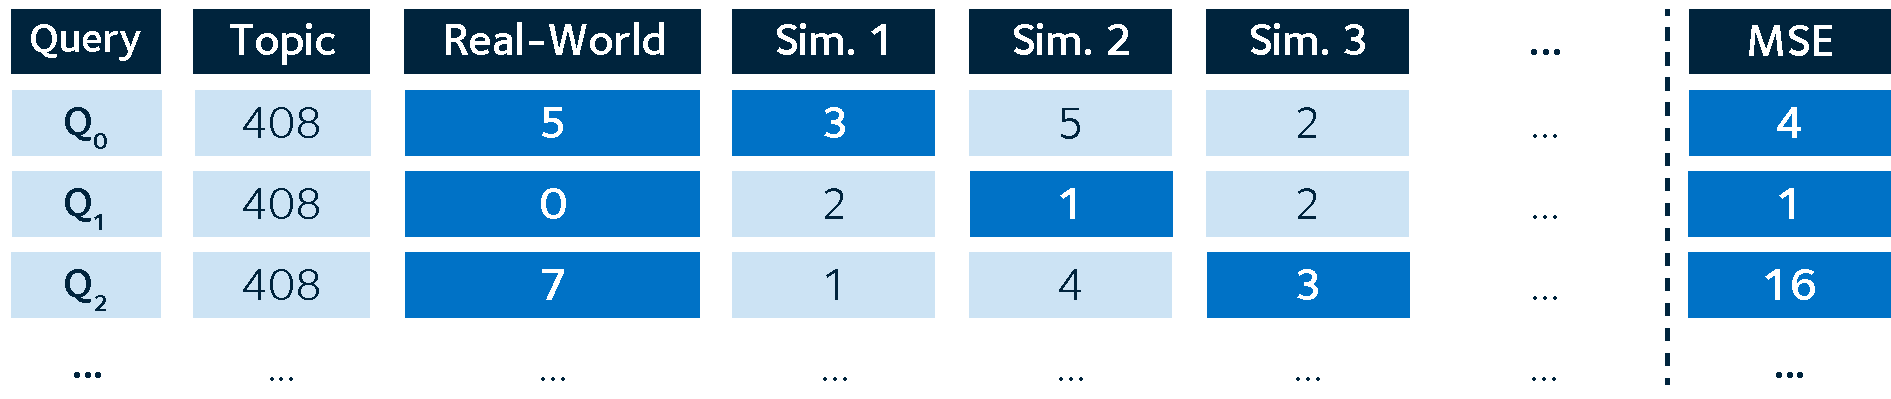
\includegraphics{figures/ch6-mse.pdf}}
    \vspace*{-8mm}
\end{figure*}

In the above, \emph{Sim. x} represents the mean value of a particular simulated searcher configuration, with the mean taken over the 50 simulated trials. For each query, the real-world click depth is shown, along with the simulated click depth from each simulated searcher trialled. The cells highlighted show what is being compared on each row -- for instance, for query $Q_0$, the real-world click depth of $5$ is compared against the \emph{Sim. 1} click depth of $3$. Considering the MSE value between the two, using the following formula:

\begin{equation*}
MSE = (\theta - \hat{\theta})^{2},
\end{equation*}

where $\theta$ denotes the real-world click depth, and $\hat{\theta}$ denotes the click depth approximation, we arrive at a MSE value of $4$. The closer the MSE value is to $0$, the better the approximation given. As such, in the above example, the compared values for $Q_1$ offer the best approximation of the actual stopping depth of the searcher. The above is just for illustration: we considered every simulated searcher, over every query. After each MSE value had been calculated, this could then be used to plot the mean depth per query across a variety of different stopping strategies. For example, recall that \blueboxbold{SS1-FIX} considers the stopping depth across a range of threshold parameter values ($x_1$), with the parameter denoting the stopping depth. The higher this value, the greater the depth per query that will be attained. By computing the MSE at each point, we then are able to determine which stopping threshold offers the best approximation of stopping behaviour, for that particular stopping strategy.

\section{Chapter Summary}
In this chapter, we have outlined the \emph{general methodology} that is used throughout the remaining contributory chapters of this thesis. As we report on two separate user studies in Chapters~\ref{chap:snippets} and~\ref{chap:diversity}, this chapter provides an overview of the common approaches followed, with unique aspects pertaining to the individual user studies discussed in the appropriate chapter. For example, implementations of the~\gls{acr:serp}-level stopping decision component are discussed in Chapter~\ref{chap:serp}.

In order to tackle the high-level research questions of this thesis, our general methodology was to first undertake a \blueboxbold{user study} that captured a variety of different behavioural, performance and user experience measures, as discussed in Section~\ref{sec:methodology:user}. The data derived from this user study was then used to ground a series of complex \blueboxbold{simulations of interaction}, attempting to mimic the behaviours exhibited by the real-world user study subjects. After discussing how we instantiated each of the different components of the~\gls{acr:csm} and \simiir~framework, we then concluded the chapter with a discussion on the two sets of simulation runs trialled, allowing us to address research questions \darkblueboxbold{HL-RQ3a} and \darkblueboxbold{HL-RQ3b}.

With the conclusion of this chapter, all the necessary groundwork has been laid to present the results of our user studies and simulations of interaction, which we begin in Part~\ref{part:context}.